%%%%%%%%%%%%%%%%%%%%%%%%%%%%%%%%%%%%%%%%%
% Masters/Doctoral Thesis 
% LaTeX Template
% Version 1.42 (19/1/14)
%
% This template has been downloaded from:
% http://www.latextemplates.com
%
% Original authors:
% Steven Gunn 
% http://users.ecs.soton.ac.uk/srg/softwaretools/document/templates/
% and
% Sunil Patel
% http://www.sunilpatel.co.uk/thesis-template/
%
% License:
% CC BY-NC-SA 3.0 (http://creativecommons.org/licenses/by-nc-sa/3.0/)
%
% Note:
% Make sure to edit document variables in the Thesis.cls file
%
%%%%%%%%%%%%%%%%%%%%%%%%%%%%%%%%%%%%%%%%%

%----------------------------------------------------------------------------------------
%	PACKAGES AND OTHER DOCUMENT CONFIGURATIONS
%----------------------------------------------------------------------------------------

\documentclass[11pt, a4paper, oneside]{Thesis} % Paper size, default font size and one-sided paper

\graphicspath{{Pictures/}} % Specifies the directory where pictures are stored

\usepackage[square, numbers, comma, sort&compress]{natbib} % Use the natbib reference package - read up on this to edit the reference style; if you want text (e.g. Smith et al., 2012) for the in-text references (instead of numbers), remove 'numbers' 
\usepackage[final]{pdfpages}
\usepackage{listings}
\usepackage{longtable}
\usepackage{multirow}
\usepackage{subcaption}

\lstnewenvironment{code}[1][]%
  {\minipage{\linewidth} 
   \lstset{basicstyle=\ttfamily\footnotesize}}
  {\endminipage}


\hypersetup{urlcolor=blue, colorlinks=true} % Colors hyperlinks in blue - change to black if annoying
\title{\ttitle} % Defines the thesis title - don't touch this

% from pandoc
\usepackage{ifxetex,ifluatex}
\usepackage{fixltx2e} % provides \textsubscript
% use upquote if available, for straight quotes in verbatim environments
\IfFileExists{upquote.sty}{\usepackage{upquote}}{}
\ifnum 0\ifxetex 1\fi\ifluatex 1\fi=0 % if pdftex
  \usepackage[utf8]{inputenc}
\else % if luatex or xelatex
  \ifxetex
    \usepackage{mathspec}
    \usepackage{xltxtra,xunicode}
  \else
    \usepackage{fontspec}
  \fi
  \defaultfontfeatures{Mapping=tex-text,Scale=MatchLowercase}
  \newcommand{\euro}{€}
\fi
% use microtype if available
\IfFileExists{microtype.sty}{\usepackage{microtype}}{}
\usepackage{color}
\usepackage{fancyvrb}
\newcommand{\VerbBar}{|}
\newcommand{\VERB}{\Verb[commandchars=\\\{\}]}
\DefineVerbatimEnvironment{Highlighting}{Verbatim}{commandchars=\\\{\}}
% Add ',fontsize=\small' for more characters per line
\newenvironment{Shaded}{}{}
\newcommand{\KeywordTok}[1]{\textcolor[rgb]{0.00,0.44,0.13}{\textbf{{#1}}}}
\newcommand{\DataTypeTok}[1]{\textcolor[rgb]{0.56,0.13,0.00}{{#1}}}
\newcommand{\DecValTok}[1]{\textcolor[rgb]{0.25,0.63,0.44}{{#1}}}
\newcommand{\BaseNTok}[1]{\textcolor[rgb]{0.25,0.63,0.44}{{#1}}}
\newcommand{\FloatTok}[1]{\textcolor[rgb]{0.25,0.63,0.44}{{#1}}}
\newcommand{\CharTok}[1]{\textcolor[rgb]{0.25,0.44,0.63}{{#1}}}
\newcommand{\StringTok}[1]{\textcolor[rgb]{0.25,0.44,0.63}{{#1}}}
\newcommand{\CommentTok}[1]{\textcolor[rgb]{0.38,0.63,0.69}{\textit{{#1}}}}
\newcommand{\OtherTok}[1]{\textcolor[rgb]{0.00,0.44,0.13}{{#1}}}
\newcommand{\AlertTok}[1]{\textcolor[rgb]{1.00,0.00,0.00}{\textbf{{#1}}}}
\newcommand{\FunctionTok}[1]{\textcolor[rgb]{0.02,0.16,0.49}{{#1}}}
\newcommand{\RegionMarkerTok}[1]{{#1}}
\newcommand{\ErrorTok}[1]{\textcolor[rgb]{1.00,0.00,0.00}{\textbf{{#1}}}}
\newcommand{\NormalTok}[1]{{#1}}
% \ifxetex
%   \usepackage[setpagesize=false, % page size defined by xetex
%               unicode=false, % unicode breaks when used with xetex
%               xetex]{hyperref}
% \else
%   \usepackage[unicode=true]{hyperref}
% \fi
% end from pandoc

\begin{document}

\frontmatter % Use roman page numbering style (i, ii, iii, iv...) for the pre-content pages

\setstretch{1.3} % Line spacing of 1.3

% Define the page headers using the FancyHdr package and set up for one-sided printing
\fancyhead{} % Clears all page headers and footers
\rhead{\thepage} % Sets the right side header to show the page number
\lhead{} % Clears the left side page header

\pagestyle{fancy} % Finally, use the "fancy" page style to implement the FancyHdr headers

\newcommand{\HRule}{\rule{\linewidth}{0.5mm}} % New command to make the lines in the title page

% PDF meta-data
\hypersetup{pdftitle={\ttitle}}
\hypersetup{pdfsubject=\subjectname}
\hypersetup{pdfauthor=\authornames}
\hypersetup{pdfkeywords=\keywordnames}



%----------------------------------------------------------------------------------------
%	TITLE PAGE
%----------------------------------------------------------------------------------------

\begin{titlepage}
\begin{center}

\textsc{\LARGE \univname}\\[1.5cm] % University name
\textsc{\Large Individual Project Report}\\[0.5cm] % Thesis type

\HRule \\[0.4cm] % Horizontal line
{\huge \bfseries \ttitle}\\[0.4cm] % Thesis title
JavaScript - Native Client Remote Procedure Calls
\HRule \\[1.5cm] % Horizontal line
 
\begin{minipage}{0.4\textwidth}
\begin{flushleft} \large
\emph{Author:}\\
Mohamed Eltuhamy % Author name - remove the \href bracket to remove the link
\end{flushleft}
\end{minipage}
\begin{minipage}{0.4\textwidth}
\begin{flushright} \large
\emph{Supervisor:} \\
\href{http://www.doc.ic.ac.uk/~cristic/}{\supname} % Supervisor name - remove the \href bracket to remove the link 
\\[0.2cm]
\emph{Co-Supervisor:} \\
\href{http://www.doc.ic.ac.uk/~ph1310/}{Petr Hosek}
\end{flushright}
\end{minipage}\\[3cm]
 
%\large \textit{A thesis submitted in fulfilment of the requirements\\ for the degree of \degreename}\\[0.3cm] % University requirement text
%\textit{in the}\\[0.4cm]
\deptname\\[2cm] % Research group name and department name
 
{\large \today}\\[4cm] % Date
%\includegraphics{Logo} % University/department logo - uncomment to place it
 
\vfill
\end{center}

\end{titlepage}

%----------------------------------------------------------------------------------------
%	DECLARATION PAGE
%	Your institution may give you a different text to place here
%----------------------------------------------------------------------------------------

% \Declaration{

% \addtocontents{toc}{\vspace{1em}} % Add a gap in the Contents, for aesthetics

% I, \authornames, declare that this thesis titled, '\ttitle' and the work presented in it are my own. I confirm that:

% \begin{itemize} 
% \item[\tiny{$\blacksquare$}] This work was done wholly or mainly while in candidature for a research degree at this University.
% \item[\tiny{$\blacksquare$}] Where any part of this thesis has previously been submitted for a degree or any other qualification at this University or any other institution, this has been clearly stated.
% \item[\tiny{$\blacksquare$}] Where I have consulted the published work of others, this is always clearly attributed.
% \item[\tiny{$\blacksquare$}] Where I have quoted from the work of others, the source is always given. With the exception of such quotations, this thesis is entirely my own work.
% \item[\tiny{$\blacksquare$}] I have acknowledged all main sources of help.
% \item[\tiny{$\blacksquare$}] Where the thesis is based on work done by myself jointly with others, I have made clear exactly what was done by others and what I have contributed myself.\\
% \end{itemize}
 
% Signed:\\
% \rule[1em]{25em}{0.5pt} % This prints a line for the signature
 
% Date:\\
% \rule[1em]{25em}{0.5pt} % This prints a line to write the date
% }

% \clearpage % Start a new page

%----------------------------------------------------------------------------------------
%	QUOTATION PAGE
%----------------------------------------------------------------------------------------

% \pagestyle{empty} % No headers or footers for the following pages

% \null\vfill % Add some space to move the quote down the page a bit

% \textit{``Thanks to my solid academic training, today I can write hundreds of words on virtually any topic without possessing a shred of information, which is how I got a good job in journalism."}

% \begin{flushright}
% Dave Barry
% \end{flushright}

% \vfill\vfill\vfill\vfill\vfill\vfill\null % Add some space at the bottom to position the quote just right

% \clearpage % Start a new page

%----------------------------------------------------------------------------------------
%	ABSTRACT PAGE
%----------------------------------------------------------------------------------------

\addtotoc{Abstract} % Add the "Abstract" page entry to the Contents

\abstract{\addtocontents{toc}{\vspace{1em}} % Add a gap in the Contents, for aesthetics

TODO Thesis abstract here.
}

\clearpage % Start a new page

%----------------------------------------------------------------------------------------
%	ACKNOWLEDGEMENTS
%----------------------------------------------------------------------------------------

\setstretch{1.3} % Reset the line-spacing to 1.3 for body text (if it has changed)

\acknowledgements{\addtocontents{toc}{\vspace{1em}} % Add a gap in the Contents, for aesthetics

TODO Acknowledgements
}
\clearpage % Start a new page

%----------------------------------------------------------------------------------------
%	LIST OF CONTENTS/FIGURES/TABLES PAGES
%----------------------------------------------------------------------------------------

\pagestyle{fancy} % The page style headers have been "empty" all this time, now use the "fancy" headers as defined before to bring them back

\lhead{\emph{Contents}} % Set the left side page header to "Contents"
\tableofcontents % Write out the Table of Contents

%\lhead{\emph{List of Figures}} % Set the left side page header to "List of Figures"
%\listoffigures % Write out the List of Figures

%\lhead{\emph{List of Tables}} % Set the left side page header to "List of Tables"
%\listoftables % Write out the List of Tables

%----------------------------------------------------------------------------------------
%	ABBREVIATIONS
%----------------------------------------------------------------------------------------

% \clearpage % Start a new page

% \setstretch{1.5} % Set the line spacing to 1.5, this makes the following tables easier to read

% \lhead{\emph{Abbreviations}} % Set the left side page header to "Abbreviations"
% \listofsymbols{ll} % Include a list of Abbreviations (a table of two columns)
% {
% \textbf{LAH} & \textbf{L}ist \textbf{A}bbreviations \textbf{H}ere \\
% %\textbf{Acronym} & \textbf{W}hat (it) \textbf{S}tands \textbf{F}or \\
% }

%----------------------------------------------------------------------------------------
%	PHYSICAL CONSTANTS/OTHER DEFINITIONS
%----------------------------------------------------------------------------------------

% \clearpage % Start a new page

% \lhead{\emph{Physical Constants}} % Set the left side page header to "Physical Constants"

% \listofconstants{lrcl} % Include a list of Physical Constants (a four column table)
% {
% Speed of Light & $c$ & $=$ & $2.997\ 924\ 58\times10^{8}\ \mbox{ms}^{-\mbox{s}}$ (exact)\\
% % Constant Name & Symbol & = & Constant Value (with units) \\
% }

%----------------------------------------------------------------------------------------
%	SYMBOLS
%----------------------------------------------------------------------------------------

% \clearpage % Start a new page

% \lhead{\emph{Symbols}} % Set the left side page header to "Symbols"

% \listofnomenclature{lll} % Include a list of Symbols (a three column table)
% {
% $a$ & distance & m \\
% $P$ & power & W (Js$^{-1}$) \\
% % Symbol & Name & Unit \\

% & & \\ % Gap to separate the Roman symbols from the Greek

% $\omega$ & angular frequency & rads$^{-1}$ \\
% % Symbol & Name & Unit \\
% }

%----------------------------------------------------------------------------------------
%	DEDICATION
%----------------------------------------------------------------------------------------

% \setstretch{1.3} % Return the line spacing back to 1.3

% \pagestyle{empty} % Page style needs to be empty for this page

% \dedicatory{For/Dedicated to/To my\ldots} % Dedication text

% \addtocontents{toc}{\vspace{2em}} % Add a gap in the Contents, for aesthetics

%----------------------------------------------------------------------------------------
%	THESIS CONTENT - CHAPTERS
%----------------------------------------------------------------------------------------

\mainmatter % Begin numeric (1,2,3...) page numbering

\pagestyle{fancy} % Return the page headers back to the "fancy" style

% Include the chapters of the thesis as separate files from the Chapters folder
% Uncomment the lines as you write the chapters
TODO: Move footnotes to references
\chapter{Introduction} 

\label{Chapter1}

\lhead{Chapter 1. \emph{Introduction}}
Over the past decades, the web has quickly evolved from being a simple online catalogue of information to becoming a massive distributed platform for web applications that are used by millions of people. Developers have used JavaScript to write web applications that run on the browser, but JavaScript has some limitations. 

One of the problems of JavaScript is performance. JavaScript is a single threaded language with lack of support for concurrency. Although web browser vendors such as Google and Mozilla are continuously improving JavaScript run time performance, it is still a slow interpreted language, especially compared to compiled languages such as C++. Many attempts have been made to increase performance of web applications. One of the first solutions was browser plugins that run in the browser, such as Flash or Java Applets. However, these have often created browser bugs and loop-holes that can be used maliciously to compromise security.

Native Client \cite{nacl} (NaCl) is a technology from Google that allows running binary code in a sandboxed environment in the Chrome browser. This technology allows web developers to write and use computation-heavy programs that run inside a web application, whilst maintaining the security levels we expect when visiting web applications.

The native code is typically written in C++, though other languages can be supported. The code is compiled and the binary application is sandboxed by verifying the code to ensure no potentially un-secure instructions or system-calls are made. This is done by compiling the source code using the gcc\footnote{The GNU Compiler Collection (gcc) is an open-source compiler that supports C, C++, and other languages \cite{gcc}} based NaCl compiler. This generates a NaCl module that can be embedded into the web page. Because no system calls can be made, the only way an application can communicate with the operating system (for example, to play audio) is through the web browser, which supports several APIs in JavaScript that are secure to use and also cross-platform. This means that the fast-performing C++ application needs to communicate with the JavaScript web application.

\lstset{language=JavaScript,caption={JavaScript code sending and receiving messages from a Native Client module},label=jsnaclexample}
\begin{code}
// Send a message to the NaCl module
function sendHello () {
  if (HelloTutorialModule) {
    // Module has loaded, send it a message using postMessage
    HelloTutorialModule.postMessage("hello");
  } else {
    // Module still not loaded!
    console.error("The module still hasn't loaded");
  }
}

// Handle a message from the NaCl module
function handleMessage(message_event) {
  console.log("NACL: " + message_event.data);
}
\end{code}


\lstset{language=C++,caption={C++ code showing the use of PostMessage and HandleMessage},label=cppnaclexample}
\begin{code}
// Handle a message coming from JavaScript
virtual void HandleMessage(const pp::Var& var_message) {
  // Send a message to JavaScript
  PostMessage(var_message);
}
\end{code}

The way Native Client modules can communicate with the JavaScript web application (and vice versa) is through simple message passing. The JavaScript web application sends a message in the form of a JavaScript string to the NaCl module. The NaCl module handles message events by receiving this string as a parameter passed into the \lstinline+HandleMessage+ function. For example, Listing \ref{jsnaclexample} shows a simplified example of how JavaScript sends a message to the NaCl module, and Listing \ref{cppnaclexample} shows how the native module handles the message and sends the same message back to the JavaScript application. This allows for straight forward, asynchronous communication between the native code and the web application. Modern web browsers support message passing using the \lstinline+postMessage+ API. This was designed to allow web applications to communicate with one or more web workers
\footnote{Web workers\cite{webworkersw3c} are scripts that run in the background of a web page, independent of the web page itself. It is a way of carrying out computations while not blocking the main page's execution. Although they allow concurrency, they are relatively heavyweight and are not intended to be spawned in large numbers. Typically a web application would have one web worker to carry out computations, and the main page to do most of the view logic (such as click listening, etc.)}. 

However, message passing puts more burden on the developer to write the required communication code between the NaCl module and the application. For example, consider a C++ program that performs some heavy computations and has functions that take several parameters of different types. To make the functionality accessible from the web application, the developer would need to write a lot of code in the \lstinline+HandleMessage+ function. A message format would need to be specified to distinguish which function is being called. Then the parameters of the function call would need to be identified, extracted, and converted into C++ types in order that the parameters are passed into the C++ function. Then a similar procedure would need to be done if the function would return anything back to the web application. 

The purpose of this project is to allow developers to easily invoke NaCl modules by creating a Remote Procedure Call (RPC) framework on top of the existing message passing mechanism. To achieve this, the developer will simply write an Interface Definition Language (IDL) file which specifies the functions that are to be made accessible from JavaScript. The IDL file will be parsed in order to automatically generate JavaScript and C++ method stubs that implement the required communication code using message passing. This is similar to how RPC is implemented in other traditional frameworks, such as ONC RPC (page \pageref{sub:oncrpc_intro}) or CORBA (page \pageref{sub:corba_intro}).

The main contributions of this project is to create a tool that parses IDL files and generates JavaScript and C++ method stubs, a message format that will be used in communication, and support libraries in JavaScript and C++ that will use message passing to do the actual communication. This will allow functions in the Native Client module to be called directly from the JavaScript application. We will evaluate how much this will help developers by seeing how many lines can be saved, in different program contexts. We will also analyse the speed and efficiency of using RPC over hand-written message passing. 

\chapter{Background}

\label{Chapter2} 

\lhead{Chapter 2. \emph{Background}} 

\section{Native Client} % (fold)
\label{sec:native_client_intro}

Native Client (NaCl) can be thought of as a new type of plugin for the Google Chrome browser that allows binary programs to run natively in the web browser. It can be used as a `back end' for a normal web application written in JavaScript, since the binary program will run much faster. A NaCl module can be written in any language, including assembly languages, so long as the binary is checked and verified to be safe by the NaCl sandbox \cite{nacl}. However, NaCl provides a Software Development Kit (SDK) that includes a compiler based on gcc that allows developers to compile C and C++ programs into binary that will work directly with the sandbox without further modifications. Thus, writing NaCl-compatible C++ programs is as easy as writing normal C++ programs with the difference between them being that the sandboxes disallow unwanted side-effects and system calls. Since many applications might want to have this type of functionality, Native Client provides a set of cross-platform API functions that achieve the same outcomes, but by communicating with the browser directly. To avoid calling NaCl syscalls directly, an independent runtime (IRT) is provided, along with two different C libraries (newlib and glibc) on top of which the Pepper Plugin API (PPAPI or `Pepper') is exposed. It can be used to do file IO, play audio, and render graphics. The PPAPI also includes the \lstinline+PostMessage+ functionality, which allows the NaCl module to communicate with the JavaScript application.

\subsection{Portable Native Client} % (fold)
\label{sub:portable_native_client}
When Native Client was first released in 2011, it allowed operating system independent binary to run in a web application. However, it produced architecture-specific applications using the same source code. These were called nexe modules. For example, it produced x86 64 bit as well as i386 binaries. However, for the developer, distributing different binaries for the same application was tedious, and architecture specific distributions go against the general trend of the truly independent web platform.

PNaCl was later introduced to solve the problem of lack of portability. Instead of producing architecture specific nexe executables, portable pexe modules are produced instead. These have a verified bitcode format. The PNaCl runtime, which runs as part of the browser, translates the bitcode into machine code. Because of their cross-platform nature, PNaCl (pexe) modules are allowed to run in Google Chrome without the user installing them, while NaCl (nexe) modules must be installed through the Chrome Web Store. However, NaCl modules allow inline assembly and different C standard library implementations, while PNaCl modules only support the newlib implementation and don't support architecture specific instructions.
% subsection portable_native_client (end)

\subsection{NaCl Modules and the Pepper API} % (fold)
\label{sub:nacl_modules_ppapi}
A Native Client application consists of the following \cite{nacloverview}:
\begin{description}
  \item[HTML/JavaScript Application:] 
  Where the user interface of the application will be defined, and the JavaScript here could also perform computations. The HTML file will include   the NaCl module by using an embed tag, e.g. \\
   \lstinline+<embed src="myModule.nmf" type="application/x-nacl" />+
  \item[Pepper API:] 
  Allows the NaCl module communicate with the web browser and use its features. Provides \lstinline+PostMessage+ to allow message passing to the JavaScript application.
  \item[Native Client Module:] 
  The binary application, which performs heavy computation at native speeds.
\end{description}

% subsection nacl_modules_ppapi (end)

\subsection{Communicating with JavaScript using postMessage} % (fold)
\label{sub:postmessage_intro}
The HTML5 \lstinline+postMessage+ API was designed to allow web workers to communicate with the main page's JavaScript execution thread. The JavaScript object is copied to the web worker by value. If the object has cycles, they are maintained as long as the cycles exist in the same object. This is known as the structured clone algorithm, and is part of the HTML5 draft specification \cite{html5w3c}. 

In a similar way, \lstinline+postMessage+ allows message passing to and from NaCl modules. However, sending objects with cycles will cause an error. NaCl allows sending and receiving primitive JavaScript objects (\lstinline+Number+, \lstinline+String+, \lstinline+Boolean+, \lstinline+null+) as well as dictionaries (key-value \lstinline+Object+ types), arrays, and \lstinline+ArrayBuffers+. ArrayBuffers are a new type of JavaScript object based on Typed Arrays \cite{typedarraysw3c} that allows the storing of binary data. 

Another key difference is that message types need to be converted into the correct type on the receiving end. For example, sending a JavaScript \lstinline+Object+ should translate into a dictionary type. The JavaScript types are dynamic in nature. A JavaScript \lstinline+Number+ object could be an integer, a float, a double, `infinity', exponential, and so on. Sending C++ data to JavaScript is simple since it is converting from a more specific type to a less specific type (e.g. from \lstinline+int+ in C++ to \lstinline+Number+ in JavaScript). But converting from a JavaScript type to a C++ type requires more thought. The PPAPI provides several functions to determine the JavaScript type (e.g. \lstinline+bool is_double()+). It also allows us to extract and cast the data into our required type (e.g. \lstinline+double AsDouble()+). From there, we can use the standard C++ type to perform the required computations.

% subsection postmessage_intro (end)

% section native_client_intro (end)

\pagebreak
\section{Remote Procedural Call (RPC)}
\label{RPCBackgroundSection} 
RPC is used to uniformly call a procedure that is on a different machine, or on the same machine but on different processes. RPC is implemented on top of a transmission protocol and should work regardless of the communication method being used. For example, we could use TCP/IP for network communications, or any Inter-Process Communication (IPC) method if the caller and callee are on the same machine but in different processes. Normally, RPC implementations would consist of the following steps, as shown in Figure \ref{fig:rpc-components}.

\begin{enumerate}
  \item The caller code is written normally, and so is the server code, but the stubs are automatically generated using interface definition files.
  \item When the remote call is made, it calls the user stub which packs the parameters and function call information into a packet.
  \item The packet gets transferred to its destination (either across the network as in Figure \ref{fig:rpc-components}, or across the processes on the same machine using IPC). This is done through the RPCRuntime, which is a library that works on both ends (caller and callee) to handle communication details.
  \item The packet is received at the callee end by the RPCRuntime. It is then passed on to the server stub.
  \item The arguments and function call information are unpacked and a normal call is made to the actual procedure.
  \item When the procedure returns, it is passed back to the server stub where it is packed and transmitted back to the caller, which unpacks it and uses the result.
\end{enumerate}

\begin{figure}
    \centering
    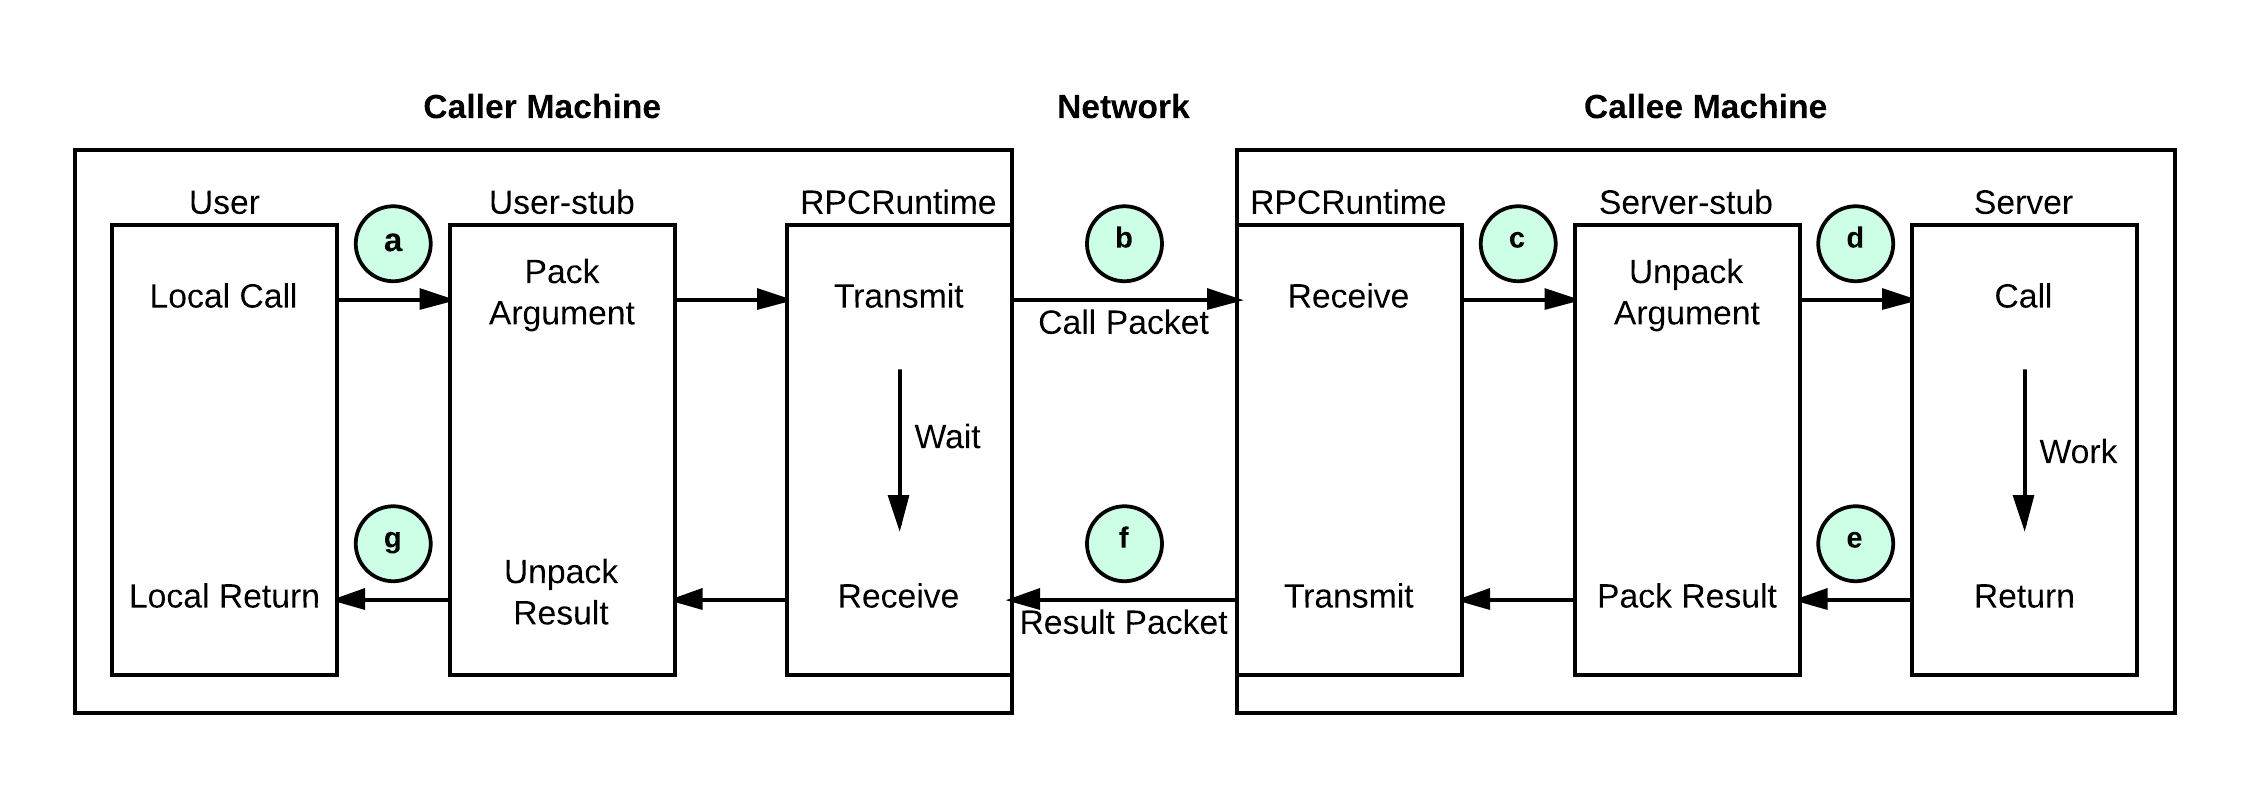
\includegraphics[bb=0 0 1270 474, width=\textwidth]{RPCDiagram_ImplementingRPC_ADBirrell_BJNelson.png} 
    \caption{The basic components of an RPC framework, from \cite{birrell1984implementing}}
    \label{fig:rpc-components}
\end{figure}

\subsection{The role of the RPCRuntime}
\label{RPCRuntimeBackgroundSection} 
The RPCRuntime is responsible for carrying out the actual communication of the RPC call information between the caller and the callee. It exists both in the caller and callee endpoints. When the caller makes a RPC call, the information is sent from the RPCRuntime sitting in the caller side, and is received by the RPCRuntime in the callee side. When the callee returns, the return data is sent from the callee's RPCRuntime to the caller's RPCRuntime.

In order to keep the context of a remote call, the RPCRuntime also sends some extra meta data along with the arguments. This meta data includes:

\begin{enumerate}
	\item A call identifier. This is used for two reasons:
	\begin{enumerate}
		\item To check if the call has already been made (i.e. to ensure no duplicate calls)
		\item To match the return value of the callee with the correct caller.
	\end{enumerate}
	\item The name of the procedure the caller is calling.
	\item The arguments (parameters) we wish to pass to the remote procedure.
\end{enumerate}

The RPCRuntime on the caller side maintains a store of call identifiers that are currently in progress. When the remote functions return, they send the same call identifier along with the return value. That call identifier is then removed from the caller's store to indicate that the remote call has completed. The call identifier is also used to implement the call semantics. Call semantics could be \emph{at least once}, where the RPC system will keep trying to call the remote procedure if the transport fails, and/or \emph{at most once}, where the system will ensure that the function is not called more than once (which is needed for nonidempotent functions).


\pagebreak
\section{RPC Implementations} % (fold)
\label{sec:rpc_implementations}

\subsection{Open Network Computing (ONC) RPC} % (fold)
\label{sub:oncrpc_intro}

ONC is a suite of software originally developed and released in 1985 by Sun Microsystems\cite{stevens2004unix}. It provides a RPC system along with an External Data Representation (XDR) format used alongside it. The ONC RPC system implements some tools and libraries that make it easy for developers to specify and use remote functions. These are:

\begin{enumerate}
	\item \textbf{RPCGen Compiler:} As mentioned earlier, the role of the user and server stubs is to pack and unpack arguments and results of function calls. To pack the arguments, the stub looks at the argument types and matches them with the number of arguments and their types of the server (callee) function definition. Thus, the stubs need to be written with knowledge of the interface of the actual procedures that will be called. We can define these interfaces in an abstract way, so that we could generate these stubs automatically even if the languages used in the different endpoints are different. In ONC RPC and many other systems, this abstract representation is in the form of an Interface Definition Language (IDL) file. When we pass the IDL file into the RPCGen compiler, it automatically generates the stubs we need to perform remote procedure calls.
	\item \textbf{XDR Routines:} These convert the types of the parameters and return values to and from the external data representation. XDR routines exist for many C types, and the system allows you to write your own XDR routines for complex types.
	\item \textbf{RPC API library:} This is an implementation that fulfils the role of the RPCRuntime described in \ref{sub:rpcruntime_background}. It provides a set of API functions that set up the lower level communication details, binding, and so on.
\end{enumerate}

Remote procedures in ONC RPC are identified by a program number, a version number, and a procedure number. There also exists a port mapper that map the program number to a port, so that several programs can run on the same remote machine. 

\subsubsection{XDR files}
\label{sec:xdrsyntax}
In ONC RPC, the XDR format is used to define RPC definitions. For example, the RPC definition in listing \ref{samplerpc} defines an interface for a simple function that takes in a character string  and returns a structure containing two fields. As discussed in \ref{sub:oncrpc_intro}, we can see the program number is \lstinline+80000+ and the procedure number of the \lstinline+generate_keypair+ function is \lstinline+1+.

\lstset{language=c,caption={An example RPC definition for a key-pair generator function},label=samplerpc}
\begin{lstlisting}
/* File: keypairgen.x */
struct key_pair_t
{
  string  public_key<500>;
  string  private_key<500>;
};

program KEYPAIRGEN_PROGRAM
{
  version KEYPAIRGEN_VERSION
  {
    /* Produce a public/private key pair using a passphrase  */
    key_pair_t generate_keypair (string) = 1;
  } = 0;
} = 80000;
\end{lstlisting}

We can use the RPCGen compiler to then create client and server stubs. Passing the definition file \verb+keypairgen.x+ (shown in listing \ref{samplerpc}) into \lstinline+rpcgen+ will produce the following files:

\begin{itemize}
	\item \textbf{keypairgen.h} The header file, which would be included in both client and server code. Includes the actual C definition of the result\_t structure we defined in the XDR.
	\item \textbf{keypairgen\_clnt.c} The client stub, which packs the parameters and uses the RPC API library to execute the actual remote procedure call.
	\item \textbf{keypairgen\_svc.c} The server stub, which uses the RPC API to set up a listener for RPC calls. RPC calls are received, parameters are unpacked, and the actual function implementation (of \lstinline+generate_keypair+) is called.
	\item \textbf{keypairgen\_xdr.c} Defines methods for packing more complex structures, such as the \lstinline+key_pair_t+ structure we defined.
\end{itemize}

Now we need to write the actual implementation of the RPC procedure we wish to call remotely, namely \lstinline+generate_keypair+. This will include the generated header file and follow the specification we defined, as shown in listing \ref{samplerpcImp}. \\


\lstset{language=c,caption={An example server-side implementation of the procedure defined in \ref{samplerpc}},label=samplerpcImp}
\begin{lstlisting}
#include "keypairgen.h"

key_pair_t *
generate_keypair_0_svc(char **argp, struct svc_req *rqstp)
{
  static key_pair_t  result;
  // TODO: Actual implementation
  return(&result);
}
\end{lstlisting}

Finally, we call the remote procedure from the client, which includes the same header file and simply calls \lstinline+generate_keypair_0+, passing in the string parameter.

% subsection oncrpc_intro (end)


%---------------------------------------------------------------------------------------------------------------------%
% CORBA
%---------------------------------------------------------------------------------------------------------------------%
\subsection{Common Object Request Broker Architecture (CORBA)} % (fold)
\label{sub:corba_intro}

CORBA is a RPC implementation introduced in 1991 by the Object Management Group (OMG) to address some issues with existing RPC implementations and provide more features for object oriented programming.

Remote method calls on objects revolve around the use of the Object Request Broker (ORB)\cite{isocorba}. A client invokes a remote object by sending a request through the ORB. The ORB locates the object on the server, and handles the communication of the remote call from the client to that object, including parameter and result packing. The client is statically aware of the objects it could invoke through the use of IDL (known as OMG IDL) stubs. These specify everything about the remote object except the implementation itself. This includes the names of classes, method interfaces, and fields. The OMG IDL is independent of any language, and bindings exist for several languages. 

Remote objects could also be invoked dynamically at runtime, as CORBA supports dynamic binding. This works by adding the interface definitions to an Interface Repository service. The implementation of the remote object is not aware how it was remotely invoked as shown in Figure \ref{fig:corba-interfaces}.

\begin{figure}
    \centering
    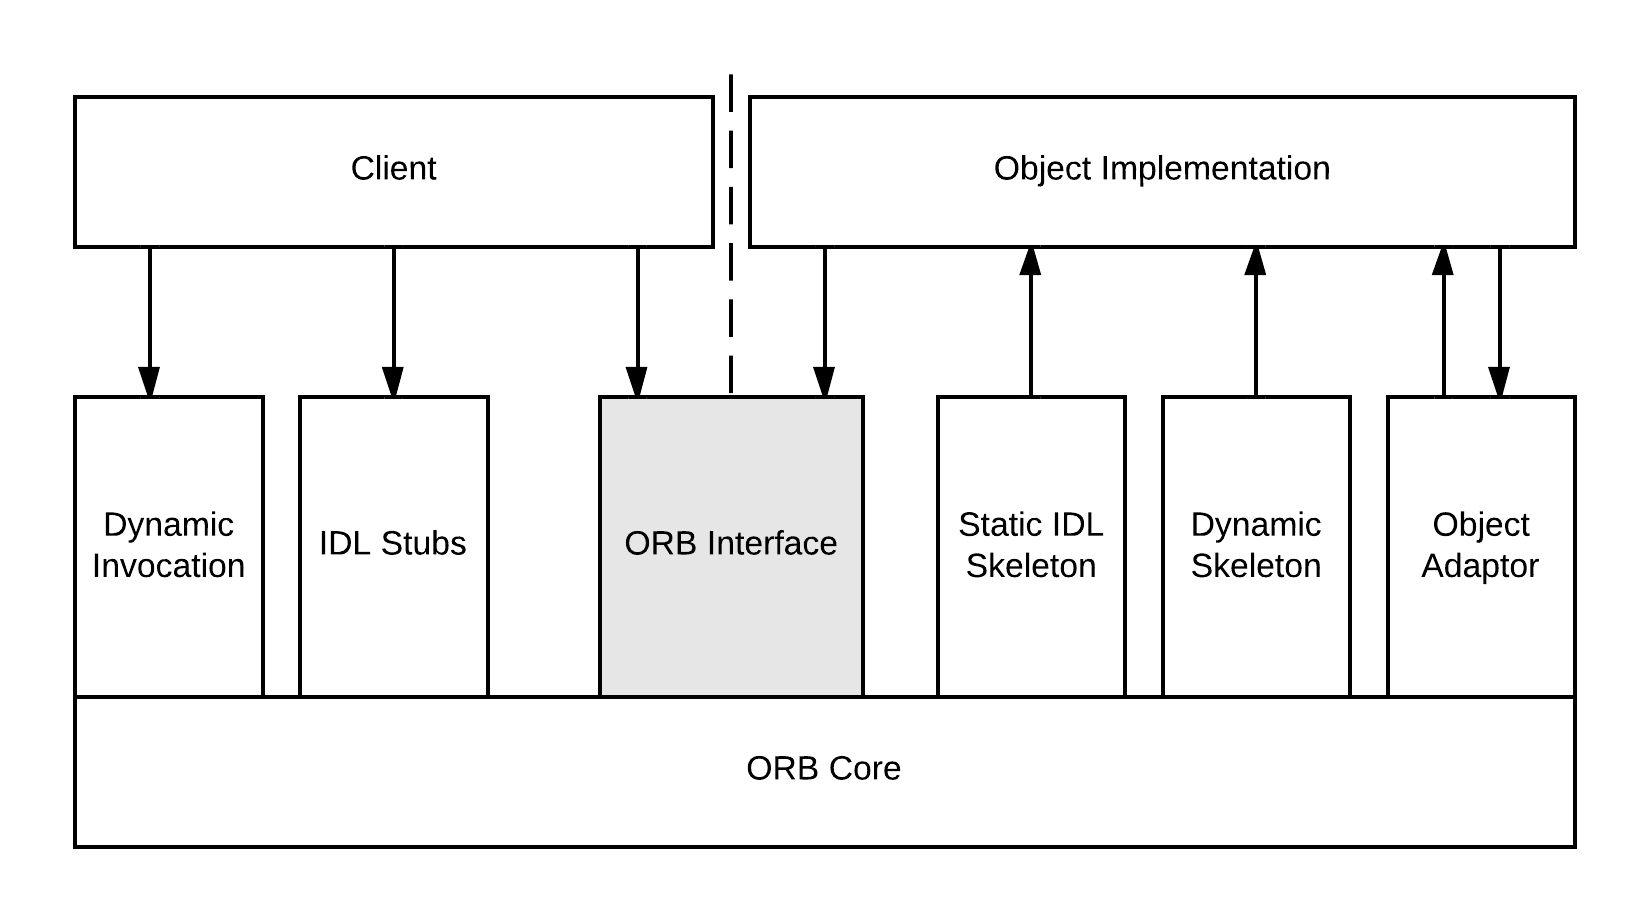
\includegraphics[bb=0 0 1074 629, width=\textwidth]{corba-client-object.png}
    \caption{Interface and Implementation Repositories in CORBA, from \cite{isocorba}}
    \label{fig:corba-interfaces}
\end{figure}

TODO: Write more about CORBA using the CORBA paper. \cite{vinoski1997corba}

% subsection corba_intro (end)


%---------------------------------------------------------------------------------------------------------------------%
% JSON-RPC and XML-RPC
%---------------------------------------------------------------------------------------------------------------------%
\subsection{JSON-RPC and XML-RPC} % (fold)
\label{sub:json_xml_rpc_intro}
XML-RPC is a simple RPC protocol which uses XML (Extended Mark-up Language) to define remote method calls and responses. It uses explicit data typing - the method name and parameters are hard-coded in the message itself. Messages are typically transported to remote servers over HTTP\footnote{Hyper-text transport protocol (HTTP) is the most common transfer protocol used by clients and servers to transfer data on the web}. Many implementations of XML-RPC exist in several different languages. 

For example, we could represent the RPC function call we defined before (Listing \ref{samplerpc}) as the XML-RPC function call shown in Listing \ref{examplexmlcall}.

\lstset{language=xml,caption={An example XML-RPC call},label=examplexmlcall}
\begin{lstlisting}
<methodCall>
  <methodName>
    generate_keypair
  </methodName>
  <params>
    <param><value><string> myPassPhraseHere </string></value></param>
  </params>
</methodCall>
\end{lstlisting}

The XML-RPC implementation could give a better interface for the XML calls. For example, run-time reflection APIs could be used to dynamically translate procedure calls into XML-RPC requests. The response from the server would also be in XML form. For example, the response for the request shown in Listing \ref{examplexmlcall} would be as shown in Listing \ref{examplexmlresponse}.

\lstset{language=xml,caption={An example XML-RPC response},label=examplexmlresponse}
\begin{lstlisting}
<methodResponse>
  <params>
    <param>
        <value>
          <struct>
            <member>
              <name>public_key</name>
              <value><string>qo96IJJfiPYWy3q3p5nvbNME87jG</string></value>
            </member>
            <member>
              <name>private_key</name>
              <value><string>IIEpAIBAAKCAQEA4eLvDruo9CswdW</string></value>
            </member>
          </struct>
        </value>
    </param>
  </params>
</methodResponse>
\end{lstlisting}

XML-RPC supports simple types like integer, double, string, boolean values. It also supports some complex types like arrays, and associative arrays (\lstinline{struct}). An example of this is in Listing \ref{examplexmlresponse}, where our structure has two keys with their respective values. Binary data can be Base64\footnote{Base64 is an encoding scheme that represents binary data as an ASCII string} encoded and sent in a \lstinline{<base64 />} tag. Because of the fixed language, XML-RPC is naturally cross-language compatible, as it is up to the two ends (client and server) to implement and use their own XML parsers and converters. Several libraries in different languages exist that do this.

XML-RPC and JSON-RPC are very similar. JavaScript Object Notation (JSON) is a simple and light-weight human-readable message format. Its advantages over XML is that it is a lot lighter and simpler. However, XML can be extended to support complex user-defined types using XML-Schemas, which is not possible directly using JSON. JSON-RPC is also a protocol and message format, for which different implementations exist. For example, we can easily represent the RPC call and response shown in Listings \ref{examplexmlcall} and \ref{examplexmlresponse} using the JSON-RPC protocol format as shown in Listing \ref{examplejsonrpc}.
\\

\lstset{language=c,caption={An example JSON-RPC request and response},label=examplejsonrpc}
\begin{lstlisting}
// JSON-RPC request:
{ 
  "jsonrpc": "2.0", 
  "method": "generate_keypair", 
  "params": ["myPassPhraseHere"], 
  "id": 1
}


// JSON-RPC response:
{
  "jsonrpc": "2.0", 
  "result": {
    "public_key": "qo96IJJfiPYWy3q3p5nvbNME87jG",
    "private_key": "IIEpAIBAAKCAQEA4eLvDruo9CswdW"
  }, 
  "id": 1
}

\end{lstlisting}

Both XML-RPC and JSON-RPC have well-defined protocols \cite{jsonrpcspec}\cite{xmlrpcspec}, and are implemented in many different languages.
% subsection json_xml_rpc_intro (end)

\subsection{WebIDL} % (fold)
\label{sub:webidl_intro}
WebIDL is a specification \cite{webidlw3c} for an interface definition language that can be used by web browsers. It is used in several projects, including Google Chrome's Blink project\footnote{\url{http://www.chromium.org/blink/webidl}}.

The WebIDL syntax is similar to ONC RPC's XDR syntax (see section \ref{sec:xdrsyntax}). Listing \ref{webIDLExample} shows the same interface as Listing \ref{samplerpc}, but this time using WebIDL.

\lstset{language=c,caption={An example interface definition written in WebIDL},label=webIDLExample}
\begin{lstlisting}
dictionary keypair {
  DOMString public_key;
  DOMString private_key;
};

interface KEYPAIRGEN {
  keypair generate_keypair(DOMString passphrase);
};
\end{lstlisting}

Just like in ONC RPC, the WebIDL files can be parsed and used to generate stub methods for the client and server. Because they are language independent, the client and server files that are generated could be in different languages. 

Open source parsers exist for WebIDL, and a standard-compliant one is provided in the Chromium project
\footnote{ \url{http://goo.gl/kAnGCU} }. 

There are also open source C++ bindings for WebIDL, such as esidl\footnote{esidl is a library provided with the es Operating System project, which is an experimental operating system whose API is written in WebIDL. The WebIDL compiler can be obtained from: \url{https://github.com/esrille/esidl}}. Similarly, bindings for JavaScript also exist\footnote{\url{https://github.com/extensibleweb/webidl.js}}. 

% subsection webidl_intro (end)

% section rpc_implementations (end)

\pagebreak
\section{Data Representation and Transfer} % (fold)
\label{sec:data_representation_and_transfer}

When designing RPC systems, the data representation of the messages being transferred, including how the parameters are marshalled, needs to be defined. This is because the client and server might have different architectures that affect how data is represented. There are two types of data representation: implicit typing and explicit typing.

Implicit typing refers to representations which do not encode the names or the types of the parameters when marshalling them. Only the values of the parameters are sent. It is up to the sender and receiver to ensure that the types being sent/received are correct, and this is normally done statically through the IDL files which specify how the message will be structured. 

Explicit typing refers to when the parameter names and types are encoded with the message during marshalling. This increases the size of the messages, but simplifies the process of de-marshalling the parameters.

This section gives an overview of some of the different message formats that can be used with RPC.


\begin{description}
	\item[XML and JSON] 
	~\\
	XML and JSON are widely used data representation formats that are supported by many languages. They are supported by default in all web browsers, which include XML and JSON parsers. XML and JSON - based RPC implementations exist, and we discuss them in Section \ref{sub:json_xml_rpc_intro}.

	Although XML and JSON are both intended to be human-readable, JSON is often more readable. JSON is also more compact, as it requires less syntax to represent complex structures, in contrast to XML which requires opening and closing tags. Here is an example of representing a phone book in XML and JSON.

	\lstset{language=c,caption={Representing a phone book using JSON},label=phonebookjson}
	\begin{code}
[
	{
		"name" : "John Smith",
		"id"   : 1,
		"phonenumber": "+447813945734"
	},
	{
		"name" : "Jane Taylor",
		"id"   : 2,
		"phonenumber": "+442383045711"
	},
]
	\end{code}
	\lstset{language=xml,caption={Representing a phone book using XML},label=phonebookxml}
	\begin{code}
<numbers type="array">
    <entry>
    	<field name="name">John Smith</field>
    	<field name="id">1</field>
    	<field name="phonenumber">+447813945734</field>
    </entry>
    <entry>
    	<field name="name">Jane Taylor</field>
    	<field name="id">2</field>
    	<field name="phonenumber">+442383045711</field>
    </entry>
</numbers>
	\end{code}

	The XML would also need to be parsed to make sense of the data. For example, a `field' tag could be parsed and converted into a C++ data structure, but that would require us to understand the structure we're using. Sometimes the structure is well defined, like in the XML-RPC protocol (see Section \ref{sub:json_xml_rpc_intro}). However, this strict parsing requirement is easier to error check, since if the XML was parsed successfully, we can be more confident that the data type is correct. 

	\item[Protocol Buffers] 
	~\\
	Google Protocol Buffers are ``a language-neutral, platform-neutral, extensible way of serializing structured data for use in communications protocols, data storage, and more", according to the developer guide\cite{protobufdev}. They are used extensively within many Google products, including AppEngine\footnote{Google AppEngine is a Platform as a Service that allows developers to run their applications on the cloud}. 

	Messages are defined in .proto files. Listing \ref{exampleproto} shows an example, adapted from the Developer Overview.
	~\\

	\lstset{language=c,caption={A .proto file},label=exampleproto}
	\begin{code}
message Person {
  required string name = 1;
  required int32 id = 2;
  optional string email = 3;

  enum PhoneType {
    MOBILE = 0;
    HOME = 1;
    WORK = 2;
  }

  message PhoneNumber {
    required string number = 1;
    optional PhoneType type = 2 [default = HOME];
  }

  repeated PhoneNumber phone = 4;
}
	\end{code}

	The .proto file is then parsed and compiled, to generate data access classes used to change the content of an instance of the representation. They also provide the methods required for serialization. These methods are shown in Listing \ref{exampleprotoserialisation}. When serialised data is converted to raw binary.

	\lstset{language=c,caption={Manipulating and serialising a .proto-generated class},label=exampleprotoserialisation}
	\begin{code}
// Serialization
Person person;
person.set_name("John Doe");
person.set_id(1234);
person.set_email("jdoe@example.com");
fstream output("myfile", ios::out | ios::binary);
person.SerializeToOstream(&output);

// De-serialisation 
fstream input("myfile", ios::in | ios::binary);
Person person;
person.ParseFromIstream(&input);
cout << "Name: " << person.name() << endl;
cout << "E-mail: " << person.email() << endl;
	\end{code}


	Many RPC implementations which use protocol buffers exist. Although Java, C++, and Python are the languages that are officially supported, people have created open source  implementations for other languages, including JavaScript\cite{protobufjs}.
\end{description}

% section data_representation_and_transfer (end)

\pagebreak
\section{Native Client Development} % (fold)
\label{sec:native_client_development}
Native Client applications are designed to be cross-platform. To provide cross-platform binaries, the Native Client SDK contains different tool chains - which include different compilers, linkers, assemblers, and other tools to build the application.

\subsection{Toolchains} % (fold)
\label{sub:toolchains}
The tool chains provided by the SDK are:
\begin{itemize}
	\item pnacl: This allows compiling C/C++ code into pnacl bitcode, as described in \ref{sub:portable_native_client} (page \pageref{sub:portable_native_client}). The pnacl toolchain uses the llvm compiler project, and the newlib and libc++ standard library implementations.
	\item nacl-gcc: This allows compiling C/C++ code into verified machine code. NaCl modules can use the newlib or glibc standard C library implementations and libc++ or libstdc++ C++ standard library implementations.
\end{itemize}

\subsubsection{Simplified Building using \lstinline+make+} % (fold)
\label{ssub:building}
The SDK also includes a Makefile called \lstinline+common.mk+ which is used by the included examples and demos to simplify the build process. This makes it easy to write an application for any of the toolchains, without worrying about compiler locations, include file paths, etc.

To specify the compiler, all that needs to be done is to specify the \lstinline+TOOLCHAIN+ environment variable. For example, running \lstinline+make TOOLCHAIN=newlib+ selects the nacl-gcc toolchain and newlib C standard library implementation.

There is also a \lstinline+CONFIG+ environment variable that can be set to specify the compiler's optimisation level. This can be \lstinline+Release+ or \lstinline+Debug+.

To illustrate the usage of \lstinline+common.mk+, listing \ref{getting_started_makefile} shows the Makefile from the SDK's getting started example.

\lstset{language=make,caption={Using the common.mk makefile, as seen in the getting started example},label=getting_started_makefile}
\begin{code}
include $(NACL_SDK_ROOT)/tools/common.mk
TARGET = part2
LIBS = ppapi_cpp ppapi pthread

CFLAGS = -Wall
SOURCES = hello_tutorial.cc

# Build rules generated by macros from common.mk:

$(foreach src,$(SOURCES),$(eval $(call COMPILE_RULE,$(src),$(CFLAGS))))

ifeq ($(CONFIG),Release)
$(eval $(call LINK_RULE,$(TARGET)_unstripped,$(SOURCES),$(LIBS),$(DEPS)))
$(eval $(call STRIP_RULE,$(TARGET),$(TARGET)_unstripped))
else
$(eval $(call LINK_RULE,$(TARGET),$(SOURCES),$(LIBS),$(DEPS)))
endif

$(eval $(call NMF_RULE,$(TARGET),))

\end{code}

Now, running \lstinline+make TOOLCHAIN=newlib CONFIG=Debug+ will compile and build the same sources for the newlib toolchain and Debug config. Running \lstinline+make TOOLCHAIN=all+ compiles and builds the same sources for pnacl, newlib and glibc.

% subsubsection building (end)

\subsubsection{Creating libraries} % (fold)
\label{ssub:creating_libraries}
In C/C++, libraries can be created using the \lstinline+ar+ and \lstinline+ranlib+ tools. This creates a \lstinline+.a+ file which can be later linked with another program. Using the Native Client SDK, this is also supported, but the locations of these tools will depend on the tool chain used.

Thankfully, the common.mk file also provides Makefile macros that make this easy. Using the LIB macro will create the static libraries and also install the libraries into the relevant SDK location. This means it is easy to link in a library for a specific tool chain all using the \lstinline+TOOLCHAIN+ and \lstinline+CONFIG+ variables.

As for dynamic libraries (\lstinline+.so+ files), these are only supported using the glibc tool chain, but \lstinline+common.mk+ takes care of this for us too, by installing the \lstinline+.so+ file if the tool chain is glibc.
% subsubsection creating_libraries (end)

% subsection toolchains (end)

\subsection{Porting existing libraries} % (fold)
\label{sub:naclports}
Many open source C and C++ libraries have been ported to use the Native Client SDK and toolchains. The Native Client team have made a simple platform called naclports to simplify the porting of existing libraries. 

Most of the time, porting an existing library is straight forward, as libraries often have generated makefiles using, for example, a \lstinline+./configure+ script, which allows specifying the required compilers, linkers, etc. needed for building the library. naclports automatically fills in these details. 

Any changes to default build process can be overridden in a script. Any changes to the code of the library can be specified in a patch file, which is applied before the library is built from the original sources.

For example, creating a NaCl port for libpng, an image processing library, is as simple as creating the \lstinline+pkg_info+ file shown in listing \ref{libpng_pkg_info} in naclports. naclports will then automatically download and install the library to the NaCl SDK. Afterwards, the libpng library used normally from any other C/C++ program.

\lstset{language=make,caption={The libpng naclport \lstinline+pkg_info+ file},label=libpng_pkg_info}
\begin{code}
NAME=libpng
VERSION=1.6.8
URL=http://download.sf.net/libpng/libpng-1.6.8.tar.gz
LICENSE=CUSTOM:LICENSE
DEPENDS=(zlib)
SHA1=a6d0be6facada6b4f26c24ffb23eaa2da8df9bd9
\end{code}

% subsection naclports (end)

\subsection{Using the Pepper Plugin API (PPAPI)} % (fold)
\label{sub:using_PPAPI}
\begin{figure}
    \centering
    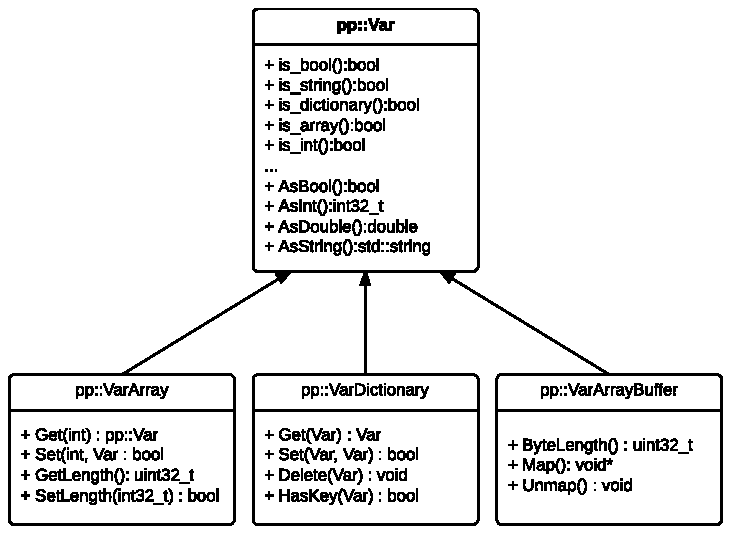
\includegraphics[width=0.8\textwidth]{pp_var-class-diagram.pdf} 
    \caption{A simplified class diagram showing the \lstinline{pp::Var} API}
    \label{fig:pp_var_api}
\end{figure}

To interface with JavaScript, Native Client provides a C and C++ library that allows developers to easily control the browser. One important class that's used in all Native Client modules is the \lstinline{pp::Instance} class, which is initialised when the embed tag is loaded in the HTML page. The class also has the \lstinline{HandleMessage} and \lstinline{PostMessage} functions, which implement message passing between the JavaScript and the C++ module. In JavaScript, JavaScript primitive types as well as reference types can be sent using postMessage. In C++, they are sent and received as \lstinline{pp::Var} objects. Figure \ref{fig:pp_var_api} shows how the \lstinline{pp::Var} classes can be used. 

Notice how C++ types can be extracted using the \lstinline{pp::Var} class. For example, we can extract a C++ \lstinline{double} from the \lstinline{pp::Var} using the \lstinline{pp::Var::AsDouble()} method. Arrays are sent and received as \lstinline{pp::VarArray} objects. JavaScript objects (dictionaries) are sent and received as \lstinline{pp::VarDictionary} objects. Binary data can be sent and received from and to the browser using the \lstinline{pp::VarArrayBuffer} class. The \lstinline{pp::VarArrayBuffer::map()} method returns a pointer to the sent binary data. 

% subsection using_PPAPI (end)

% section native_client_development (end)
\pagebreak
\section{JavaScript Development} % (fold)
\label{sec:javascript_development}
TODO: JS Dev
% section javascript_development (end)
\pagebreak
\section{Test Driven Development} % (fold)
\label{sec:test_driven_development}
Test Driven Development (TDD) is a software development approach whereby the developer writes unit-tests that describe some functionality first, then implements the functionality in order to make the tests pass.

The project includes several tests for each component of the system. Unit tests are written to test fine-grained functionality (e.g. functions), while end-to-end (E2E) tests have been written to test large parts of the system as a whole.

Because the project is implemented on both C++ and JavaScript, tests had to be written for each of these languages. Thus, the project includes the following tests:

\begin{itemize}
	\item JavaScript library tests: These test the functionality of each component of the JavaScript library. The tests run on the browser.
	\item Generator tests: These test the functionality of the JS and C++ generators.
	\item C++ library tests: These test the functionality of the C++ RPC library.
	\item E2E tests: These are test applications written to test the `full stack': starting from code generation, compilation, and all the way down to individual RPC call requests.
\end{itemize}

\subsection{Karma Test Runner} % (fold)
\label{sub:karma_test_runner}
Karma test runner\footnote{\url{http://karma-runner.github.io/}} is a library implemented at Google that makes running JavaScript tests easy. It was designed to simplify and speed up test-driven development for JavaScript. It works by letting the developer specify a configuration that states which files should be loaded, then the tests are run directly from the command line. This means the developer does not need to open a browser manually every time they want to run the tests.

Karma has been used extensively in this project to test the client side JavaScript and C++. More about configuring Karma to load C++ tests is described in the design section.
%TODO: link

% subsection karma_test_runner (end)

\subsection{JavaScript Testing Framework} % (fold)
\label{sub:js_test_framework}
Many testing frameworks exists for JavaScript. The most popular are Jasmine\footnote{\url{http://jasmine.github.io/}}, QUnit\footnote{\url{http://qunitjs.com/}} and Mocha\footnote{\url{http://visionmedia.github.io/mocha/}}. All of them support a similar set of features and APIs. 

\begin{itemize}
	\item Jasmine: %TODO
	\item QUnit:  %TODO
	\item Mocha: %TODO
\end{itemize}

In the end, I decided to use Jasmine for its straight-forward set up and easy configuration with Karma.

% subsection js_test_framework (end)

\subsection{C++ Testing Framework} % (fold)
\label{sub:cpp_testing}
Again, many unit testing frameworks and libraries exist for C++. The most popular are CppUnit, googletest, and the Boost test library.

\begin{itemize}
	\item CppUnit
	\item googletest
	\item Boost
\end{itemize}

Google Mock (gmock) is a powerful library that allows mocking classes in C++. Mocking makes it easier to test different components of a system without requiring the actual implementation. gmock can be used with any testing framework, and it is one of the most mature mocking libraries for C++ available.

I decided to use googletest for its simpler syntax, portability (as it was included with the NaCl SDK) and the fact it was easy to integrate gmock for mocking classes.

% subsection c_testing_using_gtest_and_gmock (end)

% section cpp_testing (end)
 
\chapter{Related Work} 
\label{Chapter3} 
\lhead{Chapter 3. \emph{Related Work}} 

\section{Native Client Acceleration Modules (NaClAM)} % (fold)
\label{sec:naclam}

In October 2012, John McCutchan at Google came up with the idea of using Native Client as a way to get native performance inside a normal JavaScript web application. He called it ``Native Client Acceleration Modules (NaClAM)'', with a slogan ``\emph{90\% Web App. Native Performance Where You Need It}''.

NaClAM is essentially a simple event-based RPC framework that allowed sending and receiving JavaScript objects as well as binary data. The RPC framework worked by using \emph{event listeners} and \emph{handlers} on both the JavaScript hand C++ ends. 

On the JavaScript side, a library called NaClAM.js was provided, which allowed developers to attach listeners to a particular module using the \lstinline{addEventListener(type,handler)} method. To send requests to the C++, the \lstinline{dispatchEvent} method is used. On the C++ side, messages are handled inside one overridden method called \lstinline{NaClAMModuleHandleMessage}. Here, checks are performed on the message received, and the appropriate method is called. Listing \ref{code_naclam_handle_message} shows an example of this. 

\lstset{language=C++,caption={NaClAM C++ message handler},label=code_naclam_handle_message}
\begin{code}
void NaClAMModuleHandleMessage(const NaClAMMessage& message) {
  if (message.cmdString.compare("floatsum") == 0) {
    handleFloatSum(message);
  } else if (message.cmdString.compare("addfloatarrays") == 0) {
    handleAddFloats(message);
  } else {
    NaClAMPrintf("Got message I don't understand");
  }
}
\end{code}

\subsection{Message Format} % (fold)
\label{sub:naclam_message_format}
\begin{figure}
	\centering
	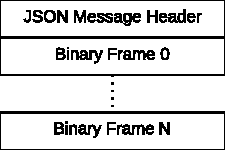
\includegraphics[width=0.3\textwidth]{naclam-msg-format.pdf} 
	\caption{A NaClAM message including binary frames}
	\label{fig:naclam_msg_format}
\end{figure}

At the message passing level, NaClAM uses JavaScript/C++ strings to transport messages. These messages hold information about the message such as the command string (like ``\lstinline{floatsum}'' in listing \ref{code_naclam_handle_message}). The strings are constructed using the jsoncpp library. 

Crucially, however, they also tell the framework how many binary \emph{frames} are expected to come after this message. Figure \ref{fig:naclam_msg_format} shows an example of a message containing $N$ frames. A frame is essentially a binary block of data sent by a separate call to \lstinline{PostMessage}. The receiver collects all the frames before triggering the event handler.

% subsection naclam_message_format (end)

\subsection{Advantages and Disadvantages} % (fold)
\label{sub:naclam_advantages_and_disadvantages}
NaClAM modules have the benefit of being simple and fast. There is a good distinction between the message information stored in the header and the message data stored as binary inside the frames. This allows developers to use the message header to implement event logic, while using the frames to transfer actual data. It also means that because the data is binary and almost no marshalling happens, the transfer speed is very fast, since binary data is \emph{shared} between JavaScript and C++.

However, there are a few issues with using NaClAM modules. The first is a lack of overall, high-level structure. The developer has to be aware and understand exactly what the framework is doing behind the scenes to write their application, which adds more burden on the developer, especially since almost no documentation is provided. The second issue is how the message header types are implemented. Although the framework allows sending application data in binary frames, the header information is sent as JSON, and is manipulated by the jsoncpp library - so another library the developer needs to get used to. Importantly, this means the developer needs to unpack and pack the data they are sending in the header section by themselves by using the jsoncpp library. Another issue is how the framework does not use a callback approach to asynchronous remote procedure calls. In other words, to `return' a value from a C++ function back to JavaScript, a \emph{different} event needs to be triggered from the C++, and handled by the JavaScript library. In other words, two different events need to be managed in both C++ and JavaScript for only one RPC call which returns data. If there are many functions like this, the developer needs to manage several different events, which is tedious. Finally, although the framework has been demoed and gained a lot of popularity, it still seems to not be well tested, as no unit tests exist for either the C++ or JavaScript implementations have been written. This makes it feel like an experimental project, rather than a full, well supported framework. 

Despite these issues, the Native Calls project was heavily influenced and inspired by the overall idea of the NaClAM project, especially its use cases and scenarios.
% subsection naclam_advantages_and_disadvantages (end)

% section naclam (end)

\section{Node.js C++ Addons} % (fold)
\label{sec:node_js_c_bindings}
Node.js is a JavaScript platform built on top of Chrome's V8 JavaScript engine that allows running JavaScript on server-side applications. Listing \ref{code_nodejs_http_server} shows an example of a node.js HTTP server.

\lstset{language=C,caption={A simple node.js HTTP server},label=code_nodejs_http_server}
\begin{code}
var http = require('http');
http.createServer(function (req, res) {
  res.writeHead(200, {'Content-Type': 'text/plain'});
  res.end('Hello World\n');
}).listen(1337, '127.0.0.1');
console.log('Server running at http://127.0.0.1:1337/');
\end{code}

Although the full JavaScript implementation is available to use in Node.js, it is possible to extend node.js by implementing addons. Addons are implemented using C++, and therefore allow developers to use efficient C++ functionality inside node.js. In fact, the C++ API allows you to wrap a C++ object with a JavaScript one. Listing \ref{code_nodejs_object_wrap_eg} shows an example of this.

\lstset{language=C++,caption={A node.js object wrapper},label=code_nodejs_object_wrap_eg}
\begin{code}
class MyObject : public node::ObjectWrap {
 public:
  static void Init(v8::Handle<v8::Object> exports);

 private:
  explicit MyObject(double value = 0);
  ~MyObject();

  static v8::Handle<v8::Value> New(const v8::Arguments& args);
  static v8::Handle<v8::Value> PlusOne(const v8::Arguments& args);
  static v8::Persistent<v8::Function> constructor;
  double value_;
};
\end{code}

In the \lstinline{Init} function, low level instructions that tell the JavaScript engine about the new object are given. In the \lstinline{New} member function, an instance of the C++ object is `wrapped' with the JavaScript object, using the node.js library. This means when we implement the \lstinline{PlusOne} method, we can `unwrap' the JavaScript object to get the C++ object instance, then perform the intended operation. Listing \ref{code_nodejs_wrapped_objects} shows how this works with the \lstinline{PlusOne} method.

\lstset{language=C++,caption={Implementing methods on wrapped objects},label=code_nodejs_wrapped_objects}
\begin{code}
Handle<Value> MyObject::PlusOne(const Arguments& args) {
  HandleScope scope;

  MyObject* obj = ObjectWrap::Unwrap<MyObject>(args.This());
  obj->value_ += 1;

  return scope.Close(Number::New(obj->value_));
}
\end{code}

Now, we can create an instance of the object in JavaScript as though it was a native JavaScript object. Listing \ref{code_nodejs_cpp_js_object} shows an example of this.

\lstset{language=C,caption={Using the C++ object from JavaScript},label=code_nodejs_cpp_js_object}
\begin{code}
var obj = new addon.MyObject(10);
console.log( obj.plusOne() ); // 11
console.log( obj.plusOne() ); // 12
\end{code}

\subsection{Advantages and Disadvantages} % (fold)
\label{sub:nodejs_cpp_advantages_and_disadvantages}
The idea of simply extending JavaScript to use your own C++ methods is powerful. We saw how the class we created in C++ can be accessed directly from JavaScript in a native way. It also means we have full control over the data the function can accept, as the actual JavaScript object reference is passed into the C++. In other words, there is no parameter marshalling - everything is native.

The obvious issue we have with C++ addons to JavaScript is how can we use them in \emph{browser} JavaScript? Well the answer is, we can't. However, we are able to set up a \emph{local} node.js server which we can communicate with using the browser. This can be done over the websocket protocol, which allow full-duplex communication over a single TCP connection. However, now the issue of parameter marshalling packing, and RPC comes to play. 


\subsection{Similar approaches in the browser} % (fold)
\label{sub:cpp_js_similar_approaches_in_the_browser}

% subsection cpp_js_similar_approaches_in_the_browser (end)
Although node.js addons do not actually solve our problem, the basic idea of them is that JavaScript is somehow \emph{extended} to allow running C++ functionality. Conventional browser plugins such as NPAPI based plugins or ActiveX browser plugins have similar interfaces. Through the plugin framework, it is possible to directly access the DOM on the page where the plugin is embedded - a bit like how this is done in node.js, as described above. 

Some frameworks such as FireBreath\footnote{\url{http://www.firebreath.org}} have been created that allow cross platform plugins that support ActiveX, NPAPI, etc. A crucial difference for us, however, is that these plugin frameworks depend on direct access to the DOM of the page in the browser. When we remove this feature, these frameworks will not work. Native Client \emph{only} allows access to the DOM through postMessage, and the data sent is \emph{passed by value}, so the data is essentially copied across to the C++ module. What this means is that the RPC framework will need to handle all marshalling as well as transport of the messages between C++ and JavaScript.
% subsection nodejs_cpp_advantages_and_disadvantages (end)

% section node_js_c_bindings (end)



\section{Apache Thrift: Cross-language services} % (fold)
\label{sec:apache_thrift_cross_language_services}
Apache Thrift is a framework that allows cross-language services development. Originally developed at Facebook, it was designed to provide reliable, efficient communication between languages and services. Many languages are supported, including C++, Java, and JavaScript. Thrift provides a cross-platform generator that can generate Thrift client and server pairs, where the client and server can be using different languages. Similar to other RPC frameworks, it uses its own IDL file format, Thrift IDL. The IDL file is used to generate code to support different languages.

\begin{figure}
    \centering
    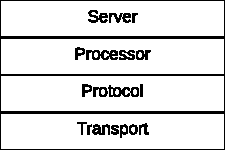
\includegraphics[width=0.3\textwidth]{thrift-stack.pdf} 
    \caption{The layers of the Apache Thrift RPC stack}
    \label{fig:thrift-stack}
\end{figure}

Thrift's implementation is based around layers in the thrift stack (Figure \ref{fig:thrift-stack}). The transport layer is responsible for the transfer of messages. The protocol layer is an interface that defines how certain data structures should be mapped into a transferable format, for example, JSON, XML, binary, etc. The process layer simply takes an input protocol, processes it using a handler, and writes to the output protocol. Finally the server sets up all the layers below it so that the system is functional as a whole.

In the following code listings, we give snippets showing how Apache Thrift is used to create a C++ server and JavaScript client. These were adapted from the original Thrift tutorial, which is available online\footnote{\url{http://thrift.apache.org/tutorial/}}.

\lstset{language=C++,caption={Thrift IDL File},label=code_thrift_idl_file}
\begin{lstlisting}
enum Operation {
  ADD = 1,
  SUBTRACT = 2,
  MULTIPLY = 3,
  DIVIDE = 4
}

struct Work {
  1: i32 num1 = 0,
  2: i32 num2,
  3: Operation op,
  4: optional string comment,
}

service Calculator extends shared.SharedService {
   void ping(),
   i32 add(1:i32 num1, 2:i32 num2),
   i32 calculate(1:i32 logid, 2:Work w)
}
\end{lstlisting}

\lstset{language=C++,caption={A Thrift C++ Server},label=code_thrift_cpp_server}
\begin{lstlisting}
class CalculatorHandler : public CalculatorIf {
 public:
  CalculatorHandler() {}

  int32_t add(const int32_t n1, const int32_t n2) {
    return n1 + n2;
  }

  int32_t calculate(const int32_t logid, const Work &work) {
    int32_t val;

    switch (work.op) {
    case Operation::ADD:
      val = work.num1 + work.num2;
      break;
    // ... other cases and implementation
    }
    return val;
  }

};

int main(int argc, char **argv) {
  // code here to set up processor, transport and protocol.

  TSimpleServer server(processor,
                       serverTransport,
                       transportFactory,
                       protocolFactory);


  server.serve();
  return 0;
}
\end{lstlisting}


\lstset{language=C,caption={JavaScript client for Thrift service},label=code_thrift_js_client}
\begin{lstlisting}
function calc() {
  var transport = new Thrift.Transport("/thrift/service/tutorial/");
  var protocol  = new Thrift.Protocol(transport);
  var client    = new CalculatorClient(protocol);

  var work = new Work()
  work.num1 = 1;
  work.num2 = 2;
  work.op = 1; //1==ADD

  var result = client.calculate(1, work);

  console.log(result); //3
  
}
\end{lstlisting}


\subsection{Advantages and Disadvantages} % (fold)
\label{sub:thrift_advantages_and_disadvantages}
Apache Thrift is a large library which seems to be well supported and used by both industry giants and the open source community. Because the Thrift IDL file is used to generate both clients and servers in more than a dozen languages, it seems that it is generic enough to be used in any language context. Thrift's implementation seems to be well structured, showing a clear separation of concerns between each component. 

However, there are a few issues with getting Thrift to work with Native Client. First, although it might be possible to implement a transport layer for thrift using postMessage in JavaScript, the C++ end (Native Client), writing a protocol for PPAPI might prove challenging. Moreover, the JSON protocol implementation uses strings instead of actual JSON objects, so this will probably impact performance, as it adds yet another marshalling step. For example, consider sending a JavaScript object from the web browser to a C++ function as a parameter. The marshalling will probably look something like this: we want to send a JavaScript Object, so Thrift for JavaScript will convert it into a JavaScript string in the protocol layer. When the JavaScript string is sent, it is marshalled by PPAPI as a \lstinline{pp::Var}, which is then marshalled as a \lstinline{std::string} using \lstinline{pp::Var::AsString()}. Thrift for C++ will then take this string and de-marshal it, in order to construct a C++ object. Finally, the C++ object is passed to the C++ concrete function. When we add on to this the fact that JavaScript strings are the slowest primitive types to transfer (according to our benchmarks in Section \ref{sec:performance_evaluation}, on page \pageref{sec:performance_evaluation}), we can see that the performance impact might actually make a big difference in an application. To avoid this, several changes will need to be made on many of the layers discussed above, which might prove to be a challenging, non-trivial task.

Finally, although unofficial port for Apache Thrift has been made for Native Client \footnote{\url{https://github.com/ahilss/thrift-nacl}}, all of the communication code is still hand coded. The performance of using Thrift for Native Client is unclear, as there is no protocol implemented using PPAPI.


% subsection thrift_advantages_and_disadvantages (end)

% section apache_thrift_cross_language_services (end)


\section{JSON-RPC Implementations} % (fold)
We briefly discussed the use of the JSON protocol RPC in background section \ref{sub:json_xml_rpc_intro} on page \pageref{sub:json_xml_rpc_intro}. Here, we discuss implementations of the protocol in JavaScript and C++.
\label{sec:json_rpc_implementations}


\subsection{JavaScript Implementations} % (fold)
\label{sub:pmrpc_json_rpc_using_postmessage}

In general, JavaScript implementations of the JSON RPC protocol are very simple, because JSON is consumed very naturally by the browser and JavaScript. Even if the JSON objects are sent and received as strings, implementations use the \lstinline{JSON.stringify(JSObject)} to turn a JavaScript object into a string, and \lstinline{JSON.parse(string)} to turn a string into a JavaScript object.

Although there are many implementations in JavaScript that are for several different domains and use cases, we discuss a simple one that uses \lstinline{postMessage} for transferring the JSON messages between browser windows, called ``PostMessage RPC (pmrpc)''. pmrpc is an open source library available on GitHub\footnote{\url{https://github.com/izuzak/pmrpc}} which aims to simplify cross-window communication by using postMessage. It shows the simplicity of remote procedure calls using JSON RPC. Listing \ref{code_prmpc_example} shows an example of using pmrpc to set up and call remote procedures between two windows.

\lstset{language=C,caption={Using pmrpc to communicate between two windows},label=code_prmpc_example}
\begin{code}
// in the callee window, expose a procedure
pmrpc.register({
  publicProcedureName : "HelloPMRPC",
  procedure : function(printParam) { alert(printParam); } 
});

// in the caller window, call the exposed procedure
pmrpc.call({
  destination : window.frames["ifr"],
  publicProcedureName : "HelloPMRPC",
  params : ["Hello World!"]
});
\end{code}
% subsection pmrpc_json_rpc_using_postmessage (end)

\subsection{C++ Implementations} % (fold)
\label{sub:jsonrpc_c_implementations}
C++ does not have native support for JSON like JavaScript, but several open source libraries exist that can read and  manipulate JSON strings. JsonCpp is one of the most popular JSON libraries for C++. We give a very brief overview of how it can be used to parse and write JSON objects. Listing \ref{code_jsoncpp_example} shows how JsonCpp is used.

\lstset{language=C++,caption={An example of using the JsonCpp library},label=code_jsoncpp_example}
\begin{code}
Json::Value root;   // will contain the root value after parsing.
Json::Reader reader;
bool parsingSuccessful = reader.parse( config_doc, root );

if(!parsingSuccessful){ /* fails to parse */ }

// Get the value of the member of root named 'encoding', 
// return 'UTF-8' if there is no such member.
std::string encoding = root.get("encoding", "UTF-8" ).asString();

// Get the value of the member of root named 'encoding', 
// return a 'null' value if there is no such member.

const Json::Value plugins = root["plug-ins"];
// Iterates over the sequence elements.
for ( int index = 0; index < plugins.size(); ++index )  
   loadPlugIn( plugins[index].asString() );
   
setIndentLength( root["indent"].get("length", 3).asInt() );
setIndentUseSpace( root["indent"].get("use_space", true).asBool() );

// don't need Json::Value constructor explicitly.
root["encoding"] = getCurrentEncoding();
root["indent"]["length"] = getCurrentIndentLength();
root["indent"]["use_space"] = getCurrentIndentUseSpace();

// jsoncpp to string
Json::StyledWriter writer;
std::string outputConfig = writer.write( root );
\end{code}

Notice how the API for JsonCpp is very similar to \lstinline{pp::Var} (see background section \ref{sub:using_PPAPI} on page \pageref{sub:using_PPAPI}). This is because \lstinline{pp::Var} and \lstinline{Json::Value} essentially do the same job - they are interfaces for JavaScript objects in C++. The crucial difference, however, is that \lstinline{Json::Value} ends up being written to a string, while \lstinline{pp::Var} objects are transferred as they are using PPAPI.

Now that we've looked at JsonCpp and how it is used, we look at an implementation of JSON RPC in C++ using JsonCpp called JsonRpc-Cpp\footnote{\url{http://jsonrpc-cpp.sourceforge.net/}}. Essentially, the framework will register methods using  the \lstinline{RpcMethod} class, which calls a function which accepts a \lstinline{Json::Value} input and a \lstinline{Json::Value} output passed by reference. Listing \ref{code_jsonrpccpphandler} shows an example of setting up a handler, adapted from the original documentation.

\lstset{language=C++,caption={Using a JsonRpc-Cpp handler},label=code_jsonrpccpphandler}
\begin{code}
class MyClass
{
   public:
     void Init()
     {
       RpcMethod* method = new RpcMethod<MyClass>(
           *this, &MyClass::RemoteMethod, // sets up pointer to C++ method
           std::string("remote_method"),  // the json-rpc "method"
           std::string("Description"));   // optional description
       m_handler.AddMethod(method);
     }

     bool RemoteMethod(const Json::Value& msg, Json::Value& response)
     {
       // do stuff
     }

   private:
     Handler m_handler;
};
\end{code}
% subsection jsonrpc_c_implementations (end)

\subsection{Advantages and Disadvantages} % (fold)
\label{sub:jsonrpc_advantages_and_disadvantages}
Many JSON RPC implementations for several languages exist\footnote{\url{http://en.wikipedia.org/wiki/JSON-RPC}}, including C++ and JavaScript as we have seen. The JSON-RPC protocol is very simple, and for most use cases, it is efficient and adequate. Although JSON RPC has a well defined protocol, it can be extended for specific implementations. Finally, JSON RPC does not need the messages to be sent and received as strings (although human-readability of the messages can be a bonus). We can use any other format to marshal and de-marshal a JSON RPC message. Some of these formats are discussed in background section \ref{sec:data_representation_and_transfer} on page \pageref{sec:data_representation_and_transfer}.

JSON RPC JavaScript implementations are simple enough to be implemented and tested in JavaScript to work for any specific project. So although libraries in JavaScript exist, implementing it for JavaScript to work with a different project structure / architecture should be not too difficult. As for C++ implementations, many if not all use the JsonCpp project. None available are implemented for \lstinline{pp::Var}. So to get JSON RPC to work with \lstinline{pp::Var}, an implementation will need to be written from scratch to use \lstinline{pp::Var}. This is also not too difficult, since as we've seen, \lstinline{Json::Value} and \lstinline{pp::Var} have similar APIs.

% subsection jsonrpc_advantages_and_disadvantages (end)

% section json_rpc_implementations (end)
\chapter{Design and Implementation}
\label{Chapter4}
\lhead{Chapter 4. \emph{Design and Implementations}} 
This section describes the design and implementation of the RPC framework and generators.

\section{RPC Framework} % (fold)
\label{sec:rpc_framework_structure}

The structure of the RPC framework is based around the notion of layers. 
Each layer solves a particular task, in order to achieve the goal of getting from a JavaScript stub to a C++ function, and back. Listing \ref{structurediagram} shows the overall structure and interactions of each layer.

The advantages of this approach is that each layer is independent of the other. For example, if we choose a different RPC schema (i.e. something other than JSON RPC), we could easily replace the JSON RPC layer. Or, if we choose to have the C++ function on the server instead of as a Native Client module, we can easily change the transport layer to use AJAX requests or Web Sockets. 


The other advantage to this approach is that because the layers are independent and each layer has a simple interface, each layer can easily be tested. For example, to test the implementation of the run time layer, we can easily mock the JSON RPC layer, since we know its public interface.

In the end, we have four layers: the stub layer, runtime layer, JSON RPC layer and transport layer. Each layer is described in detail below.

\lstset{language=c,caption={A layered approach to RPC},label=structurediagram}
\begin{code}
TODO: Turn it into a real diagram.
+-------------------------------------------------------------------+
|                           NaClRPCModule                           |
|-------------------------------------------------------------------|
|                                                                   |
|                                                                   |
|     +-------------------------------------------------------+     |
|     |+-----------------------------------------------------+|     |
|     || +--------------------+ Stub +----------------------+|| 1   |
|     |+-----------------------------------------------------+|     |
|     +-------------------------------------------------------+     |
|                 +                      ^            ^             |
|                 |                      |            |             |
|                 |callRPC               |successCB   |errorCB      |
|                 |                      |            |             |
|                 v                      +            +             |
|     +-------------------------------------------------------+     |
|     |                        Runtime                        | 2   |
|     +-------------------------------------------------------+     |
|      +          +        +                ^           ^           |
|      |          |        |                |handle     |           |
|      |send      |send    |send            |Callback   |handle     |
|      |Callback  |Error   |Request         |/handleCall|Error      |
|      v          v        v                +           +           |
|     +-------------------------------------------------------+     |
|     |                        JSONRPC                        | 3   |
|     +-------------------------------------------------------+     |
|      +         +         +                ^                       |
|      |         |         |                |                       |
|      |sendRPC  |sendRPC  |sendRPC         |handleRPCCallback      |
|      |Callback |Error    |Request         |/ handleRPCCall        |
|      v         v         v                +                       |
|     +-------------------------------------------------------+     |
|     |                       Transport                       | 4   |
|     +-------------------------------------------------------+     |
|         +        +       +                ^                       |
|         |        |       |                |                       |
|         |        |       |                |                       |
|         |on      |load   |postMessage     |handleMessage          |
|         |        |       |                |                       |
|         v        v       v                +                       |
|     +-------------------------------------------------------+     |
|     |+-----------------------------------------------------+|     |
|     ||+-------------------+ NaClModule +------------------+|| 5   |
|     |+-----------------------------------------------------+|     |
|     +-------------------------------------------------------+     |
|                                                                   |
+-------------------------------------------------------------------+
\end{code}


\subsection{Transport layer} % (fold)
\label{sub:transport_layer_design}
The role of the transport layer is to implement the transportation of messages. Messages could be anything, JavaScript objects, strings, or even binary data. Moreover, the receiver could be anything - a node.js server, or a Native Client module. Finally, the transport could use any transport mechanism - web sockets, HTTP/AJAX, WebRTC, postMessage, etc.

The important thing is that the transport must provide:
\begin{itemize}
	\item An asynchronous API (should be non-blocking)
	\item The following public API:
	\begin{itemize}
		\item a \lstinline+send+ function, that accepts a payload of any type.
		\item a constructor which sets a message handler.
		\item the message handler must be invoked when a message is received. 
	\end{itemize}
\end{itemize}

The reason this approach was taken was to allow any possibility of executing remote procedure calls. It also allows the transport layer to be testable, since no concrete implementations of the layers above or below the transport layer need to be provided to test the functionality of the transport layer.


\subsubsection{Implementing the Transport Layer in JavaScript} % (fold)
\label{ssub:implementing_the_transport_layer_in_javascript}
To implement the transport layer using a Native Client module, we first encapsulate the details of a Native Client module into its own class, called \lstinline{NaClModule}. This class essentially does all the DOM manipulation for a module. To explain this, consider how a Native Client module is normally embedded in the page (as described in the background section \ref{sub:nacl_modules_ppapi} on page \pageref{sub:nacl_modules_ppapi}). The module is embedded onto the page using an \lstinline{embed} tag. The \lstinline{src} attribute points to the location of the NaCl Manifest - which tells the browser which (p)nacl executable to load. For example, \lstinline{<embed src="myModule.nmf" type="application/x-nacl" />}. The \lstinline{type} attribute tells the browser what MIME type the executable is. This could take values of either \lstinline{x-nacl} for NaCl modules or \lstinline{x-pnacl} for PNaCl modules. 

All this detail is configured through the NaClModule constructor, which takes in an object for configuration. In other words, the same \lstinline{embed} tag is created (but not actually placed on the page \emph{yet}), using the following code:

\begin{code}
var myModule = new NaClModule({
  src: 'rpc-module.nmf', 
  name: 'rpc', 
  id: testModuleId, 
  type: 'application/x-pnacl'
});
\end{code}

However, much of the details of this can be `inferred' using the name of the module:

\begin{code}
var myModule = new NaClModule({"name": testModuleId});
// creates an embed tag with the same attributes
\end{code}

The attributes are inferred by using the NaClConfig global object, or a default config object if one does not exist. TODO: Examples of attribute inference using config.

Once a NaClModule is constructed, it can be loaded using the \lstinline{load} method, which can take in an optional callback function as a parameter. The load method essentially inserts the \lstinline{embed} element into the page. Event handlers can be registered with the module by using the \lstinline{on} method. For example:

\begin{code}
var myModule = new NaClModule({"name": testModuleId});
myModule.on('load', function(){...});
myModule.on('message', function(){...});
myModule.on('crash', function(){...});
...
\end{code}

TODO: Class diagram showing NaClModule and Transport.

The NaClModule class therefore makes it easy to create and alter the HTML embed tag using only JavaScript. 

Now, the transport layer encapsulate a NaClModule object, which is used as a low-level communication object in order to send and receive messages. 
% subsubsection implementing_the_transport_layer_in_javascript (end)

\subsubsection{Implementing the Transport Layer in C++} % (fold)
\label{ssub:implementing_the_transport_layer_in_cpp_}
Since the C++ module is a singleton, the structure of the transport in C++ is a lot simpler. Essentially, the transport is a class that extends the \lstinline{pp::Instance} class provided by the PPAPI, which we use to send and receive messages using \lstinline{pp::Instance::PostMessage} and \lstinline{pp::Instance::HandleMessage}. These methods are overridden in order to link the transport with the layer above.

TODO: Class diagram showing Transport extending pp::Instance.


% subsubsection implementing_the_transport_layer_in_cpp_ (end)

% subsection transport_layer_design (end)

\subsection{RPC layer} % (fold)
\label{sub:json_rpc_layer_design}
The RPC Layer is responsible for validating messages sent and received by the transport. 

Messages \emph{received} by the transport could either be RPC \emph{requests}, \emph{responses}, or \emph{errors}. If a message is one of these three, it should forward the message to the layer above (the \emph{runtime}). If a message is not one of these three possibilities, the message should be ignored as it is not a RPC message.

TODO: Diagram showing flow of messages handled and how they are filtered using the RPC Layer.

The RPC layer can also provide RPC \emph{send} functions, that allow messages to be sent to the layer below. It allows RPC requests, responses and errors to be sent.

TODO: Diagram showing flow of messages sent and how they are filtered using the RPC Layer.

Therefore, the RPC layer has the following API:
\begin{itemize}
	\item a \lstinline+handleMessage+ function, which accepts a payload and is called by the Transport layer when a message is received. \lstinline+handleMessage+ should filter through the messages received to categorise them as requests, responses or errors. Depending on which type of message it is, the layer can call different methods of the layer above.
	\item a \lstinline+sendRequest+ function, which validates messages to be sent as requests, and forwards it down to the transport layer to be sent.
	\item a \lstinline+sendResponse+ function, which validates messages to be sent as responses, and forwards it down to the transport layer to be sent.
	\item a \lstinline+sendError+ function, which validates messages to be sent as errors, and forwards it down to the transport layer to be sent.
\end{itemize}

\subsubsection{Choosing a protocol} % (fold)
\label{ssub:choosing_a_protocol}
We decide to use the JSON RPC 2.0 protocol. TODO: reasons + alternatives.
% subsubsection choosing_a_protocol (end)

\subsubsection{Implementing the JSON RPC Layer} % (fold)
\label{ssub:implementing_the_jsonrpc_layer}
To implement the API discussed above for JSON RPC, we first need to implement validators for messages. These determine what kind of message it is - request, response, error, or none. This is done on both the JavaScript and C++ implementations, as both will have to use the protocol. Then, when a message is received, the layer simply uses these validators to check what kind of message it is. At the same time, it extracts the relevant information about the message. For example, if it is a request, it extracts the method name, parameters, etc. 

To implement the JSON RPC protocol validators, we adhere closely to the specification. Detailed unit tests are written, including passing and failing cases. The validator is then written. This is done for both the C++ and JavaScript implementations.

As well as this, some helper functions were written to create valid RPC requests, responses, and errors.

TODO: Class diagrams showing public API.

On the C++ side, a RPCRequest object is created. The RPCRequest object encapsulates generic (i.e. not necessarily JSONRPC specific) information about a RPC call. This is passed by reference to the layers that need it, so that the validation and extraction only happens once.

TODO: Show how RPCRequest is used between layers, instead of generic `message' objects.

% subsubsection implementing_the_jsonrpc_layer (end)

% subsection json_rpc_layer_design (end)

\subsection{RPC Runtime layer} % (fold)
\label{sub:rpc_runtime_layer_design}
The main job of the runtime layer is to coordinate RPC requests and responses. As described in the background section \ref{sub:rpcruntime_background} (page \pageref{sub:rpcruntime_background}), the runtime does this by keeping track of RPC requests, and matching the requests with the responses by the use of a call identifier.

The API the runtime provides is therefore as follows:
\begin{itemize}
	\item send functions, that call the layer below.
	\begin{itemize}
		\item \lstinline+sendRequest = function(method, parameters, successCB, errorCB)+ this will give the request an ID, then keep track of that ID and the callback functions.
		\item \lstinline+sendResponse = function(id, result)+ this will just construct a response message and send it to the layer below.
		\item \lstinline+sendError = function(id, errorCode, errorMessage, errorData)+ will construct an error message and send it to the layer below.
	\end{itemize}
	\item handler functions (\lstinline+handleRequest+, \lstinline+handleResponse+, \lstinline+handleError+). The runtime will match the response's identifier with a previously sent request identifier. If a callback was provided, the callback will be called.
\end{itemize}

\subsubsection{Implementing the runtime layer} % (fold)
\label{ssub:implementing_the_runtime_layer}
The role of the runtime is different depending on the caller and the callee. Due to time constraints, the runtime has only been implemented for a JavaScript caller (client), and a C++ callee (server). However, the implementation is very similar, as it is only a language difference (in other words, the implementation in JavaScript will be the same as the implementation in C++ and vice versa).

We first consider the implementation of the caller's RPC runtime, implemented in JavaScript. TODO.

For the callee's RPC runtime, written in C++, the implementation involves finding a function. TODO. 
% subsubsection implementing_the_runtime_layer (end)

% subsection rpc_runtime_layer_design (end)

\subsection{Stub Layer} % (fold)
\label{sub:stub_layer_design}
Finally, the stub layer is just a wrapper over the runtime layer's API, so that functions can be called `natively' from within the language. The stub layer also performs parameter type checking and marshalling.

\subsubsection{Implementing the stub layer} % (fold)
\label{ssub:implementing_the_stub_layer}

% subsubsection implementing_the_stub_layer (end)
% subsection stub_layer_design (end)

% section rpc_framework_structure (end)

\newpage

\section{WebIDL Bindings} % (fold)
\label{sec:webidl_bindings}

In order to automatically generate stubs for JavaScript and C++ that allows communication between the two languages, an independent language, WebIDL, is used to define types and interfaces which will be used by both JavaScript and C++.

\begin{code}
TODO: make this an actual diagram.
C++   <->   JS

______________
|    WebIDL   |
|_____________|
  |         |
  v         v
 C++  <->  JS
\end{code}

The reason why this is needed is because JavaScript and C++ have entirely different type systems, and because the communication is two-way, we can't simply map a C++ type into a JavaScript type. Moreover, if the RPC framework were to be completely language independent, we would need a mapping between every languages type into a JavaScript type. Therefore, to generalise, WebIDL gives an intermediary type interface so that other languages can communicate with JavaScript. The WebIDL types and syntax is defined as a standard, and gives EcmaScript bindings. In other words, the conversion between WebIDL and JavaScript types is defined in the standard. It is then up to the developer of the other language to define a binding from that language to WebIDL.

In this section, we mention the C++ WebIDL bindings used in the Native Calls project, and the design decisions behind them.

The implementation challenges involved in implementing these bindings are discussed at a later chapter.

\subsection{Modules, Interfaces, and Functions} % (fold)
\label{sub:modules_and_interfaces}
In Native Calls, we make a distinction between `modules' and `interfaces'. Essentially, a module contains several interfaces. And an interface contains several function definitions.

When we define a module, we must define all the interfaces, type definitions, and dictionaries for it in the same generator call. The definitions could be in different IDL files.

In JavaScript, a module is represented as an object which has a property for each interface that module defines. Then, each interface has a property for each function that interface defines. 

In C++, a module is represented as a class, which sets up the module. When setting up the module, each function interface is added. An IDL interface is represented by a C++ header file. The header file defines each function that is in the interface.

% subsection modules_and_interfaces (end)

\subsection{Number and String Types} % (fold)
\label{sub:number_types}
WebIDL defines a number of numeric types, and also provides the JavaScript bindings for each type. The table below (TODO: give ref) shows the numeric types and their bindings in C++.

\begin{table}[h]
\begin{tabular}{l|lll}
\textbf{WebIDL Type} & \textbf{Min int} & \textbf{Max int} & \textbf{C++ Type}  \\ \hline
byte                 & $-2^{7}$         & $2^{7}-1$        & int8\_t            \\
octet                & $0$              & $2^{8}-1$        & uint8\_t           \\
short                & $-2^{15}$        & $2^{15}-1$       & int16\_t           \\
unsigned short       & $0$              & $2^{16}-1$       & uint16\_t          \\
long                 & $-2^{31}$        & $2^{31}-1$       & int32\_t           \\
unsigned long        & $0$              & $2^{32}-1$       & uint32\_t          \\
long long            & $-2^{63}$        & $2^{63}-1$       & int64\_t           \\
unsigned long long   & $0$              & $2^{64}-1$       & uint64\_t          \\
float                &                  &                  & float              \\
double               &                  &                  & double           
\end{tabular}
\end{table}

It can be observed that the integer types are represented in C++ with the size information in it, even though C++ has equivalent type names for each of the WebIDL integer types. For example, C++ supports the \lstinline{short} type, but we explicitly decide to represent \lstinline{short} as \lstinline{int16_t}. The reason why explicit size information is included in the type is because of different implementations of certain types. For example, depending on the C++ standard library implementation we use, a \lstinline{long} can be represented in 32 bits or 64 bits. But because WebIDL explicitly defines the actual size of the integer types, to stick to the standard, we can't tolerate this variation. For this reason, we use the explicit size types as shown above. This issue does not arise for \lstinline{float} and \lstinline{double} types as both C++ and JavaScript adhere to the IEEE 754 format.

Another interesting issue to note is that the bindings for large number types, such as \lstinline{long long}, are represented in JavaScript by the \emph{closest} numeric value. But because all JavaScript numbers are represented by 64 bit IEEE 754 (`double') types, the largest number that can be represented in JavaScript is actually $2^{53}-1$. This means that often the conversion between the WebIDL type and the JavaScript binding is \emph{lossy}, in the sense that it is not a one-to-one mapping. Although it would have been possible to overcome this issue by creating or using JavaScript `BigNumber' library classes, I decided to adhere to the specification, using the lossy conversion. This was for a couple of reasons:

\begin{itemize}
	\item Forcing the JavaScript user to use a number library is bad, as it adds more dependencies and is not conventional JavaScript e.g. the BigNumber library will have a different API to normal JavaScript numbers, and certain operations, such as addition, will not work properly.
	\item Using a different implementation, the RPC library could represent all data as \emph{binary}. JavaScript supports binary data in the form of ArrayBuffers.
	\item It is fairly unlikely that the developer would want to send back such large numbers to the JavaScript, and since the developer is developing for the web platform, they should be aware of JavaScript's limitations - including numeric type support.
\end{itemize}

To represent string types, the \lstinline{DOMString} WebIDL type is converted to the JavaScript \lstinline{string} type, as defined in the standard. As for the C++ binding, the \lstinline{std::string} class was chosen to represent DOMString. The alternative was to represent strings as character array buffers (\lstinline{char[]}). I decided to use the \lstinline{std::string} class for the following reasons:

\begin{itemize}
	\item JavaScript uses unicode (utf8) for strings. The developer would need to do some encoding/decoding to handle unicode characters, which might not fit in a byte.
	\item Simplicity: The PPAPI supports an \lstinline{AsString()} method on \lstinline{pp::Var} objects, which extracts the string value as a \lstinline{std::string} object.
	\item C++ developers use \lstinline{std::string} when they can. \lstinline{std::string} allows conversion to C strings using the \lstinline{c_str()} method.
\end{itemize}

% subsection number_types (end)

\subsection{Dictionary Types} % (fold)
\label{sub:dictionary_types}
The WebIDL standard defines the binding of a WebIDL dictionary to be a JavaScript Object with the keys being the identifier names of each dictionary member, and values being of the member's type. For example, Listing \ref{code_webidl_dictionary_example} shows an example of a dictionary definition in WebIDL and the corresponding JavaScript object according to the specification.

\lstset{language=C,caption={A WebIDL dictionary and its JavaScript binding},label=code_webidl_dictionary_example}
\begin{code}
// WebIDL
dictionary myObject {
  double id;
  DOMString name;
};

// Example JavaScript object
var myObj = {
  id: 31,
  name: "John Smith"
}
\end{code}

When a JavaScript object (and therefore a WebIDL dictionary) is sent to the NaCl module, it is represented in PPAPI as a \lstinline{pp::VarDictionary} object. \lstinline{pp::VarDictionary} allows extracting keys and values as \lstinline{pp::Var}. See background section \ref{sub:using_PPAPI} on page \pageref{sub:using_PPAPI} for more details.

We now consider how we can represent dictionaries in C++. The obvious approach is to represent a dictionary as a C \lstinline{struct}. The fields of the struct will have corresponding names and types as defined in the dictionary (TODO, show example). The advantage of this is that the object passed to the C++ programmer will be a normal C++ struct. However, it will impact performance, since each field of the struct will need to be individually converted. In fact, this makes marshalling dictionaries the slowest conversion, according to the benchmarks (see section \ref{sec:performance_evaluation}, page \pageref{sec:performance_evaluation}).

However, other approaches are possible. One alternative is we could have simply passed the \lstinline{pp::VarDictionary} object to the developer, without modifying it. The advantage of doing this is that it will simplify the C++ RPC library and therefore make it faster to send and receive complicated structures. However, there are a few problems with this approach:

\begin{itemize}
	\item The C++ developer is now exposed to PPAPI. This adds a learning curve, as it is another library that the C++ developer would have to get used to in order to write their module.
	\item The C++ developer will need to do all the type marshalling by themselves. This renders the dictionary type definition that they wrote in WebIDL useless, and adds more burden on the developer.
	\item The use of \lstinline{pp::VarDictionary} is actually an implementation detail of the RPC library. In other words, we simply use this as a way of transporting the data from JavaScript to C++. Perhaps someone could write another implementation that uses full binary transfer for example, using Protocol Buffers (see background section \ref{sec:data_representation_and_transfer}, page \pageref{sec:data_representation_and_transfer}). In that case, passing the \lstinline{pp::VarDictionary} to the developer would actually be more burden on the library, and probably impact performance.
\end{itemize}

Another approach is to represent a dictionary as a \lstinline{std::map}. The advantage of this is that the map can be added to and deleted from dynamically and unlike structs, if a field is not specified, data is not allocated for it. The problem with \lstinline{std::map} however is that the keys and values of the map have strict types. If the values have the same type, then a map will do fine. But what about if the values have different types, such as in the example in Listing \ref{code_webidl_dictionary_example}? The only way around this is by using wrapper types. For example, using \lstinline{pp::Var} again to represent the actual value, so the \lstinline{std::map} will be from \lstinline{std::string} keys to \lstinline{pp::Var} values. But again, this means the developer will have to de-marshal the \lstinline{pp::Var} to a standard library type, and this can get tedious when the value type is complex, for example, with multiple nested dictionaries.

In the end, we take the approach of individually, recursively de-marshalling the \lstinline{pp::VarDictionary} into a struct type, as a trade off of simplicity and developer friendliness to performance.
% subsection dictionary_types (end)

\subsection{Sequence Types} % (fold)
\label{sub:sequence_types}
In WebIDL, there are two ways of specifying a collection of types: sequence types (\lstinline{sequence<T>}) and array types (\lstinline{T[]}). The difference, according to the specification, is that a sequence type is \emph{passed by value} - meaning it is copied when passed into a function. Array types are passed by reference. 

Since \lstinline{postMessage} only transfers objects and values by value (i.e. structures are recursively copied), our RPC framework only supports sequence types. However, in JavaScript, they are represented in the same way (i.e. Array objects).

In C++, there are many ways of representing WebIDL sequence types, but we can assume we have two options: using an array structure, or a standard library template class such as \lstinline{std::vector}. We compare each approach below.

The advantage of using an array is that we do not need to use an extra library, and it might be faster for large arrays. The problem of using arrays is that anywhere we use the array, we will need to also pass its length. This can get tedious, especially if we have a function that accepts many parameters. To overcome this, it is possible to send the length of the array with the actual array by augmenting the array after a designated terminator element, such as a NULL or zero element. For example, to specify the array \lstinline{[1,2,3,4]}, we send \lstinline{[1,2,3,4,NULL,4]}. The \lstinline{4} after the \lstinline{NULL} element is the length of the array. The problem with this, however, is we need some kind of encoding scheme to ensure that the terminator and length elements do not get counted as actual array elements. For some array types, an encoding might not exist. Moreover, processing will need to be done in order for the developer to get the length of an array, thus the developer would need to get used to another library that is not standard C++.

The advantage of using a vector is that they are dynamic and they encapsulate the length of the vector. This means they are easy to both use and marshal. The disadvantage is that we're forcing the user to use the std::vector library. There are cases where the developer just wants an array.

In the end, I decided to go for the vector approach, for the following reasons:

\begin{itemize}
	\item The performance is nearly the same, since we allocate the size of the vector before using it. Also, regardless of the approach taken, it will take O(n) time to marshal and demarshal the array, since it needs to be converted to/from a \lstinline{pp::VarArray}.
	\item If the developer requires an array buffer, they can use the \lstinline{std::vector::data()} method to get a pointer to the vector's internal buffer.
	\item Vectors are generally how C++ developers represent collections of items, so most of the time it is fine to use the \lstinline{std::vector} library.
\end{itemize}

\subsubsection{Transferring contiguous number types as binary} % (fold)
\label{ssub:transferring_binary}
TODO: Move this to future work section

So far we have been discussing how to transfer a sequence of any type. This is represented in WebIDL as \lstinline{sequence<T>}, where \lstinline{T} could be any type, including dictionary types. But there is one case where it makes sense to send the data as binary data, through the use of ArrayBuffers. This is when we want to send a contiguous array of numeric type, for example, an array of floats. 

Sending binary data in that case is efficient for two reasons. The first is the fact you don't need to marshal the data into a \lstinline{pp::VarArray} type, since the binary buffer can be sent directly using the \lstinline{pp::VarArrayBuffer} class. The second reason is how binary data is transferred in NaCl. When we send an ArrayBuffer to/from JavaScript, instead of the data being copied, it is shared. Only when the data is written to does the data get copied. This makes transferring ArrayBuffers very efficient - instead of O(n) time, it will probably take O(1) time.

Now, considering the performance gains, if we decide to send and receive contiguous number arrays as ArrayBuffers, a few questions arise. The first is how will the data be represented in JavaScript, and whether or not this representation makes sense in every context. The answer is that in JavaScript, the data will need to be sent and received as an \lstinline{ArrayBuffer}. It's difficult to do anything with an ArrayBuffer though, so in JavaScript, a few more classes were made to help with reading buffers of certain types. These are called ArrayBufferViews. Currently available ArrayBufferViews are \lstinline{Int8Array}, \lstinline{Int16Array}, \lstinline{Int32Array}, \lstinline{Float32Array}, and \lstinline{Float64Array}, and also their unsigned counterparts. These classes allow accessing the data of a buffer as though it was a normal JavaScript array (TODO, show example). So, when we relate these ArrayBufferViews to IDL types, these make sense for byte, short, long, float, and double WebIDL types. The \lstinline{long long} type will be unsupported, but that is understandable, considering JavaScript's number size limitations (as described earlier). In conclusion, the answer to the first question is ``the binary data will be represented in JavaScript as an appropriate ArrayBufferView, and this representation makes sense for most number array types''.

The second question is \emph{when} do we send binary data? To answer the question, we consider when it's possible to send arrays of numbers in general:

\begin{itemize}
	\item As a parameter
	\item As a result
	\item Embedded inside a dictionary or array
\end{itemize}

We could choose to send and receive binary for \emph{all} the above scenarios, or some. To figure out when to send, we need to run some benchmarks to find how much of a performance improvement it might give.

The third question is how do we accept binary data in C++? The possibilities are either to accept it as a buffer, or a vector. As discussed earlier, however, accepting it as a buffer is problematic since we need to provide the length of the array. Luckily, we can easily and efficiently construct a vector with the same data, by providing a pointer to the data in the constructor of the vector. (TODO: give example). When sending it back, we use the \lstinline{std::vector::data()} method to efficiently get a pointer to the buffer, that we can then use to send.

The fourth and final question we need to ask is how the data is transferred from C++ to JavaScript. The answer is through the \lstinline{pp::VarArrayBuffer} interface. But there arises a problem, to do with copying memory. TODO. Go into details:
\begin{itemize}
	\item Show example.
	\item memcpy is slow.
	\item possible solution: only transfer binary when we know its size. We know its size from WebIDL.
\end{itemize}

% subsubsection transferring_binary (end)

% subsection sequence_types (end)

\subsection{Implementation in C++} % (fold)
\label{sub:webidl_implementation_in_cpp_}
TODO: Discuss parameter marshalling here.
% subsection webidl_implementation_in_cpp_ (end)

\subsection{Implementation in JavaScript} % (fold)
\label{sub:webidl_implementation_in_javascript}
TODO: Discuss parameter type checking here.
% subsection webidl_implementation_in_javascript (end)

% section webidl_bindings (end)

\newpage

\section{Generating RPC Code} % (fold)
\label{sec:generating_rpc_code}
To convert from a WebIDL file to a JavaScript and C++ RPC library, we need four main ingredients:

\begin{itemize}
	\item WebIDL type bindings to JavaScript and C++
	\item The WebIDL file(s) that define the types and interfaces of our module
	\item A WebIDL parser
	\item A generator that produces the relevant JavaScript and C++ files
\end{itemize}

In the previous section, we discussed the WebIDL bindings. In this section, we discuss the parser and generator needed to produce the relevant code.

\subsection{WebIDL Parser} % (fold)
\label{sub:webidl_parser_design}
The WebIDL parser takes as input a WebIDL file, and returns as output an Abstract Syntax Tree (AST) representation of the file. For more information about how parsers work, please read the background section \ref{sec:parsing_and_generating} on page \pageref{sec:parsing_and_generating}. 

Several open source WebIDL parsers exist, so we had a choice of using an existing parser or building our own. The advantage of building our own is that we can define the format of the AST so that it can be used directly with our generator. The disadvantage is the time and effort involved in writing the parser, as well as updating it if the WebIDL specification changes. The advantages of using an existing parser is that it will be kept relatively up to date and probably more stable, as most available parsers are unit tested to ensure they work properly. An existing parser will also be more complete, meaning they support most if not all of the WebIDL syntax and specification. For these reasons, we decided to use an existing WebIDL parser. But there was a few popular parsers to choose from. We compare and contrast the different implementations below.

\begin{itemize}
	\item Open source browser vendor implementations such as Chromium's Blink WebIDL parser\cite{chromiumwebidlparser} or Mozilla's WebIDL Parser\cite{mozillawebidlparser}.
	\item Robin Berjon's WebIDL2.js\cite{berjonwebidljs}.
\end{itemize}

The advantages of using either the Chromium or Mozilla parser is that we know it's used in an actual web browser implementation. Therefore, they are reliable and are probably maintained to be up to date with the specification. Both of these implementations are written in Python, so will run fast. However, the disadvantages are that both have very little to no documentation, and this makes both of them hard to work with. Because they are embedded in the source code of another project, it is difficult to include them in our project without copying the source code and versioning the file in our project. This means every time the parser is updated, we have to update the file separately.

The advantages of using the WebIDL2.js parser is that it is a node.js package which can be easily added as a dependency. This means we don't need to worry about updating it in our source code. Also, the parser has detailed documentation about how the abstract syntax tree is defined. This is useful for our generator. Although the parser isn't written by a browser vendor, it is well tested against the actual WebIDL specification. In fact, it is written by Robin Berjon at W3C, so we can be confident that the parser will work well at least for the majority of cases. The disadvantages is that it might be slightly slower, although this has not been measured and is not noticeable. 

In the end, I decided to go for WebIDL2.js because of its good documentation. I found the parser in JavaScript a bit easier to work with, especially since the unit tests for the generator are written in JavaScript too - so we ended up with a common testing language for the whole project.



% subsection webidl_parser_design (end)

\subsection{Code Generators} % (fold)
\label{sub:code_generators_design}
The generator essentially does the reverse of a parser - it takes in an AST and returns a string representing the relevant code. However, sometimes the AST information was not in the format which we required, so we do a single pass through the AST, augment it, then use the augmented AST to generate the code. Figure \ref{fig:generator-diagram} shows an illustration of this.

\begin{figure}
    \centering
    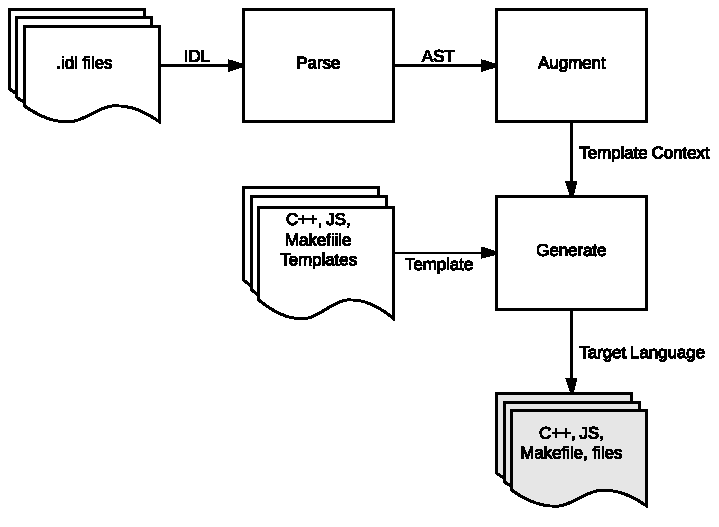
\includegraphics[width=0.9\textwidth]{generator.pdf} 
    \caption{Flow diagram showing the role of the generator}
    \label{fig:generator-diagram}
\end{figure}

We use the augmented AST as a \emph{context} to be passed to the template engine. We also add some helper functions on top of the template engine, to simplify the actual template. The template engine then uses the context to substitute the relevant strings into the correct places. For example, Listing \ref{code_template_context_eg} is a context that is used with the template shown in Listing \ref{code_template_eg} to generate the output shown in Listing \ref{code_template_output}. The rest of the code generator implementation is essentially augmenting the context to allow easy access for the template engine to generate all the files we needed.

Because the parser we used produces an AST in JavaScript, it made sense to have the generator in JavaScript too. This means we had to find a JavaScript template engine. There is more than a dozen template engine available to choose from, however, to simplify the templates and make them as human-readable as possible, we decided to limit our search only to templates with simple markup and logics. One template notation stood out, mustache\cite{mustache}. Mustache is an elegant, simple, templating language used across many languages. We decided to go with it because of its good documentation on its notation, its popularity, and its simplicity. However, several implementations of mustache existed. There was mustache.js\cite{mustachejs}, handlebars\cite{handlebarsjs}, and hogan\cite{hoganjs} by twitter. After considering each implementation, we found that they were very similar. We decided to choose hogan for its simplicity, speed, and extra features.

\lstset{language=C,caption={An example of a template context},label=code_template_context_eg}
\begin{code}
{
  timestamp: "Thu May 08 2014 21:38:16 GMT+0100 (BST)",
  moduleName: "Bullet",
  dictionaries: [{
    name: "XYZ",
    members: [
      { name: "x", STDTypeName: "float"},
      { name: "y", STDTypeName: "float"},
      { name: "z", STDTypeName: "float"}
    ]
  }]
}
\end{code}

\lstset{language=C,caption={An example of a template},label=code_template_eg}
\begin{code}
/* AUTOMATICALLY GENERATED ON {{timestamp}} */

#ifndef PPRPCGEN_{{moduleName}}_TYPES_H_
#define PPRPCGEN_{{moduleName}}_TYPES_H_

#include <string>
#include <vector>

namespace pprpcgen{
{{#dictionaries}}
typedef struct {
  {{#members}}
  {{^typeIsSequence}}{{STDTypeName}}{{/typeIsSequence}}
  {{#typeIsSequence}}std::vector<{{STDTypeName}}>{{/typeIsSequence}}
  {{name}};
  {{/members}}
} {{name}};

{{/dictionaries}}

}

#endif /* PPRPCGEN_{{moduleName}}_TYPES_H_ */

\end{code}

\lstset{language=C,caption={An example of the output of the generator},label=code_template_output}
\begin{code}
/* AUTOMATICALLY GENERATED ON Fri Jun 06 2014 20:11:41 GMT+0100 (BST) */

#ifndef PPRPCGEN_Bullet_TYPES_H_
#define PPRPCGEN_Bullet_TYPES_H_

#include <string>
#include <vector>

namespace pprpcgen{

typedef struct {
  float x;
  float y;
  float z;
} XYZ;

}

#endif /* PPRPCGEN_Bullet_TYPES_H_ */

\end{code}

% subsection code_generators_design (end)

% section generating_rpc_code (end)



\newpage

\section{Creating a testing framework} % (fold)
\label{sec:creating_a_testing_framework}
TODO.
% section creating_a_testing_framework (end) 
\chapter{Evaluation}
\label{Chapter5}
\lhead{Chapter 5. \emph{Evaluation}} 

The project has a qualitative evaluation as well as a quantitative evaluation.

The qualitative part is to do with how ``developer friendly'' the system is, as a whole. To measure it, we look at the code written by the developer, as well as the learning curve required to write a complete library from JavaScript to C++.

The quantitative part is to do with the performance characteristics of the RPC library. To measure it, we measure the average time it takes to do a native computation, the time spent in the RPC library code, and the time spent in the JavaScript library code. Therefore, we can calculate roughly how much of an overhead using the library will impact on the performance.

To study these two characteristics in a real world scenario, we will use two applications:

\begin{itemize}
	\item \emph{Bullet Physics}: A rigid-body physics simulation using the bullet physics\cite{bulletphysics} library
	\item \emph{Oniguruma}: A regular expression engine written in C++ using the Oniguruma\cite{oniguruma} library.
\end{itemize}

We also measure the general performance of the framework by the use of micro benchmarks.

The section gives the results as well as implementation details of both the qualitative and quantitative evaluation of the project. In the end, we analyse the overall performance and usability of the RPC framework, and compare it to other currently available methods.

\section{Performance Testing Environment} % (fold)
\label{sec:performance_testing_environment}
To test the framework and applications, we use the following machine specification:
\begin{itemize}
  \item Processor: 2.3 GHz Intel Core i7 (1 processor, 4 cores)
  \item Memory: 8GB 1600 MHz DDR3. 256KB L2 cache per core; 6 MB L3 cache
  \item Graphics: NVIDIA GeForce GT 650M 1024 MB
  \item OS: Mac OS X 10.9.3
  \item Google Chrome version: 35.0.1916.153 (Official Build 274914) 
  \item V8 version: 3.25.28.18
  \item Blink version: 537.36 (@175075)
  \item PPAPI version: 34
\end{itemize}

We use Benchmark JS \cite{benchmarkjs} to easily and accurately measure the amount of time taken to run JavaScript code. Benchmark JS uses high-resolution timers (microsecond precision) and automatically runs the function we wish to test enough times so that it returns statistically significant results. 
% section performance_testing_environment (end)

\section{Application Performance Evaluation} % (fold)
\label{sec:application_performance_evaluation}
\subsection{Bullet Physics Performance} % (fold)
\label{sub:bullet_physics_performance}
The simplest way to measure how well the physics engine performs using Native Calls RPC is to analyse the frames per second (FPS) for a range of scenes of varying complexity. We identify what the biggest impact to the FPS is by measuring how long it takes to make a request and get a response for each frame rendered. We also measure how long it takes to perform the actual simulation step. Finally, we compare these measurements with the original implementation, which was implemented using Native Client Acceleration Modules and tweaked for performance using ArrayBuffers.

\subsubsection{Setup} % (fold)
\label{ssub:bullet_performance_setup}
To test the implementation, we use seven physics scenes. A screenshot of each scene is shown in Figure \ref{fig:bullet_screenshots}. Apart from the Jenga scenes, each scene starts with all the objects falling from the sky and crashing on the ground.

We measure three things - the frame rate, the simulation time, and the round trip time. To measure the frame rate, we simply add to a total of frames requested. A frame is requested by the browser automatically in order to achieve a frame rate of 60 frames per second. This is done using the \lstinline{window.requestAnimationFrame} API, which conveniently takes the computation time for rendering and processing the frame into account. This is why the frame rate drops when the round trip time and simulation time increases. We measure the total simulation time inside the C++ application by taking time stamps between and after the simulation step and calculating the difference. We send it back with the results every time we do the simulation. Finally, we calculate the round trip time by taking timestamps before and after the RPC call and taking a difference. We average all this data over a period of one second and send it to be plotted.

For each second, the average time per frame is calculated. This is the inverse of frames per second, and we call this period the \emph{frame time}. During that time, a RPC request is made and a response is received. We call the period between making a request and receiving a response the \emph{RPC time}. We calculate these times and average them for each second for a period of 20 seconds - the \emph{elapsed time}. Figure \ref{fig:frame-time-vis} shows a visualisation of this terminology.

The graph is plotted in real time in the browser, but we make sure not to use the same \lstinline{window} object - as this will impact JavaScript performance and give us skewed results. Instead, we send the data to be plotted in a different window - which in Chrome corresponds to a different process. HighCharts was chosen to quickly and easily create the realtime graph with very little configuration.

The actual implementation of the RPC library for the physics simulation is discussed in the qualitative evaluation section \ref{sub:implementation_bullet_evaluation} on page \pageref{sub:implementation_bullet_evaluation}.

\begin{figure}
    \centering
    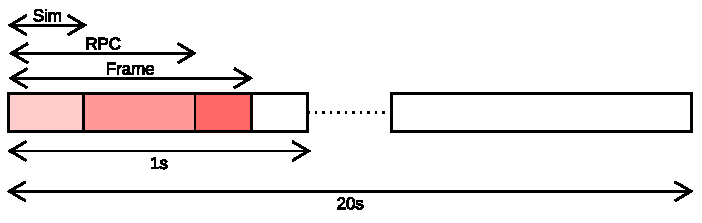
\includegraphics[width=0.7\textwidth]{FrameTimeVisualisation.pdf} 
    \caption{A graphical representation showing the times measured.}
    \label{fig:frame-time-vis}
\end{figure}

\begin{figure}
        \centering
        \begin{subfigure}[b]{0.45\textwidth}
                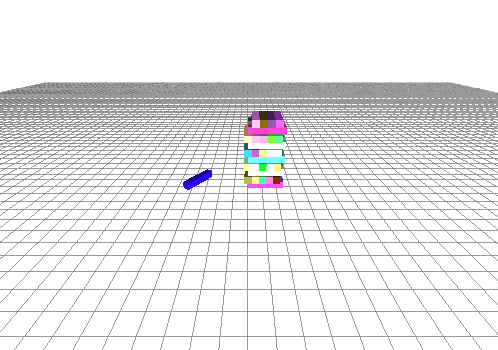
\includegraphics[width=\textwidth]{jenga_10.png}
                \caption{Jenga 10}
                \label{fig:screenshot_jenga_10}
        \end{subfigure}%
        ~ %add desired spacing between images, e. g. ~, \quad, \qquad, \hfill etc.
          %(or a blank line to force the subfigure onto a new line)
        \begin{subfigure}[b]{0.45\textwidth}
                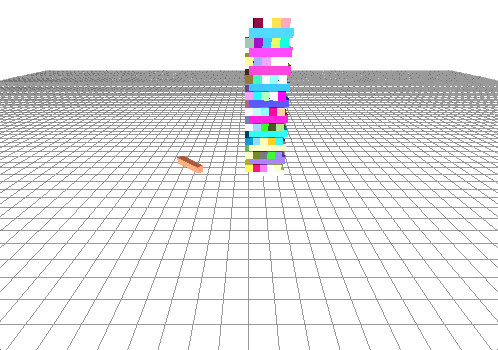
\includegraphics[width=\textwidth]{jenga_20.png}
                \caption{Jenga 20}
                \label{fig:screenshot_jenga_20}
        \end{subfigure}
        ~ %add desired spacing between images, e. g. ~, \quad, \qquad, \hfill etc.
          %(or a blank line to force the subfigure onto a new line)
        \begin{subfigure}[b]{0.45\textwidth}
                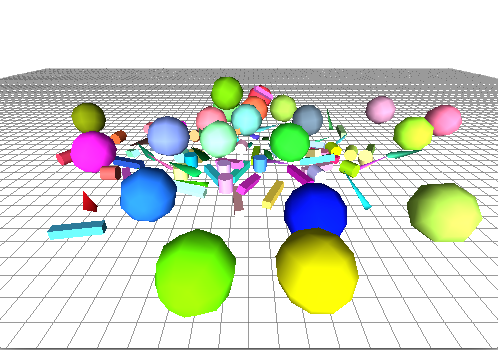
\includegraphics[width=\textwidth]{random_shapes.png}
                \caption{Random Shapes}
                \label{fig:random_shapes}
        \end{subfigure}
        ~ %add desired spacing between images, e. g. ~, \quad, \qquad, \hfill etc.
          %(or a blank line to force the subfigure onto a new line)
        \begin{subfigure}[b]{0.45\textwidth}
                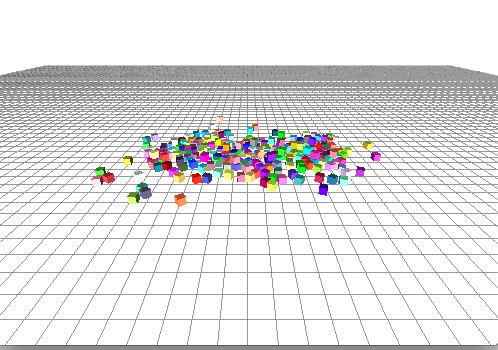
\includegraphics[width=\textwidth]{cubes_250.png}
                \caption{250 Cubes}
                \label{fig:cubes_250}
        \end{subfigure}
        \begin{subfigure}[b]{0.45\textwidth}
                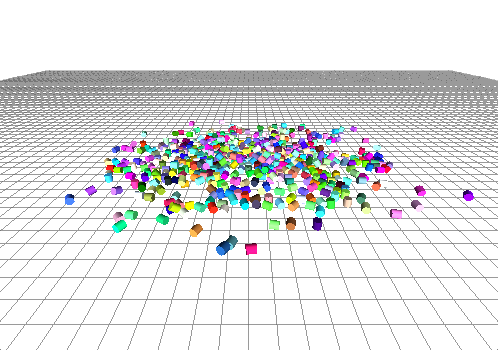
\includegraphics[width=\textwidth]{cylinders_500.png}
                \caption{500 Cylinders}
                \label{fig:cylinders_500}
        \end{subfigure}%
        ~ %add desired spacing between images, e. g. ~, \quad, \qquad, \hfill etc.
          %(or a blank line to force the subfigure onto a new line)
        \begin{subfigure}[b]{0.45\textwidth}
                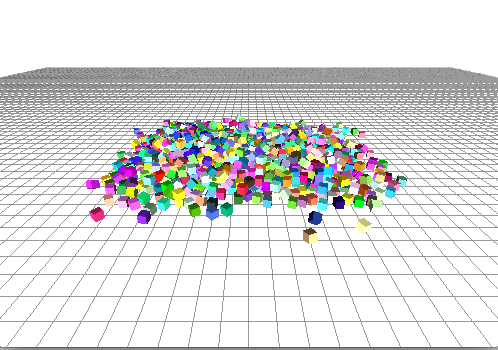
\includegraphics[width=\textwidth]{cubes_1000.png}
                \caption{1000 Cubes}
                \label{fig:cubes_1000}
        \end{subfigure}
        ~ %add desired spacing between images, e. g. ~, \quad, \qquad, \hfill etc.
          %(or a blank line to force the subfigure onto a new line)
        \begin{subfigure}[b]{0.45\textwidth}
                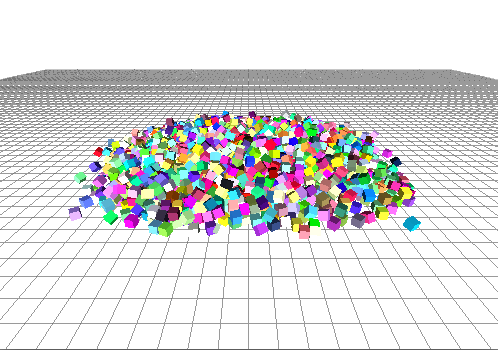
\includegraphics[width=\textwidth]{cubes_2000.png}
                \caption{2000 Cubes}
                \label{fig:cubes_2000}
        \end{subfigure}
        \caption{The bullet physics scenes used in the benchmark}\label{fig:bullet_screenshots}
\end{figure}


% subsubsection bullet_performance_setup (end)

\subsubsection{Results and comparison} % (fold)
\label{ssub:results_bullet_physics_performance}

\begin{table}[h]
    \begin{subtable}[h]{\textwidth}
        \centering
\begin{tabular}{l|lll|lll|lll|lll}
\multirow{3}{*}{Scene} & \multicolumn{9}{l|}{Time / ms}                                                          & \multicolumn{3}{l|}{\multirow{2}{*}{FPS}} \\ \cline{2-10}
                       & \multicolumn{3}{l|}{Frame} & \multicolumn{3}{l|}{RPC} & \multicolumn{3}{l|}{Simulation} & \multicolumn{3}{l|}{}                     \\ \cline{2-13} 
                       & $\mu$     & Max     & Min     & $\mu$     & Max    & Min    & $\mu$       & Max       & Min      & $\mu$          & Max          & Min          \\ \hline
A                      & 17       & 18     & 16     & 17       & 18    & 16    & 0.11       & 0.13     & 0.10    & 60            & 61          & 55          \\
B                      & 17       & 18     & 16     & 17       & 18    & 16    & 0.35       & 2.93     & 0.08    & 60            & 61          & 56          \\
C                      & 17       & 17     & 16     & 17       & 17    & 16    & 0.45       & 0.90     & 0.23    & 60            & 61          & 59          \\
D                      & 17       & 21     & 16     & 17       & 21    & 16    & 0.67       & 1.80     & 0.20    & 59            & 61          & 48          \\
E                      & 21       & 23     & 17     & 21       & 24    & 17    & 2.46       & 5.73     & 1.08    & 49            & 58          & 44          \\
F                      & 39       & 45     & 17     & 38       & 43    & 17    & 10.80      & 14.56    & 0.11    & 25            & 60          & 22          \\
G                      & 72       & 91     & 34     & 73       & 91    & 34    & 23.73      & 41.08    & 0.91    & 14            & 29          & 11         
\end{tabular}
        \caption{Using Native Calls}
    \end{subtable}
    ~
    \begin{subtable}[h]{\textwidth}
        \centering
\begin{tabular}{l|lll|lll|lll|lll}
\multirow{3}{*}{Scene} & \multicolumn{9}{l|}{Time / ms}                                                          & \multicolumn{3}{l|}{\multirow{2}{*}{FPS}} \\ \cline{2-10}
                       & \multicolumn{3}{l|}{Frame} & \multicolumn{3}{l|}{RPC} & \multicolumn{3}{l|}{Simulation} & \multicolumn{3}{l|}{}                     \\ \cline{2-13} 
                       & $\mu$     & Max     & Min     & $\mu$     & Max    & Min    & $\mu$       & Max       & Min      & $\mu$          & Max          & Min          \\ \hline
A                      & 17       & 18     & 16     & 17       & 18    & 16    & 0.13       & 0.14     & 0.12    & 60            & 61          & 55          \\
B                      & 17       & 18     & 16     & 17       & 18    & 16    & 0.38       & 3.37     & 0.10    & 60            & 61          & 57          \\
C                      & 17       & 17     & 16     & 17       & 20    & 16    & 0.60       & 0.93     & 0.27    & 60            & 61          & 59          \\
D                      & 17       & 19     & 16     & 17       & 20    & 17    & 1.14       & 1.87     & 0.22    & 60            & 61          & 52          \\
E                      & 17       & 18     & 16     & 17       & 26    & 16    & 2.64       & 5.82     & 0.97    & 60            & 61          & 55          \\
F                      & 19       & 21     & 17     & 19       & 24    & 17    & 12.06      & 15.49    & 1.09    & 53            & 59          & 48          \\
G                      & 35       & 40     & 17     & 35       & 42    & 18    & 30.77      & 37.93    & 8.86    & 29            & 58          & 25         
\end{tabular}
        \caption{Using NaClAM}
    \end{subtable}
\caption{Time measurements for the bullet physics demo, using different implementations}
\label{table:bullet_performance}
\end{table}


Table \ref{table:bullet_performance} shows the results of the measurements taken during the simulation every second, over a duration of 20 seconds. Figure \ref{fig:bullet_screenshots} shows which scene corresponds to which capital letter (for example, scene `E' is referring to the simulation of 500 cylinders).

Because the simulation is affected by time, the table shows the range of values taken for each measurement.

We can see that scenes A, B, C, D, and E have roughly similar results for both implementations. Scenes F and G show some more interesting results. Figures \ref{fig:bullet_graph_cyl500}, \ref{fig:bullet_graph_cube1000}, and \ref{fig:bullet_graph_cube2000} show some plots showing how the simulation time and frame time change per second for scenes E, F and G respectively, using the Native Calls and NaClAM implementations.

\begin{figure}
        \centering
        \begin{subfigure}[b]{\textwidth}
                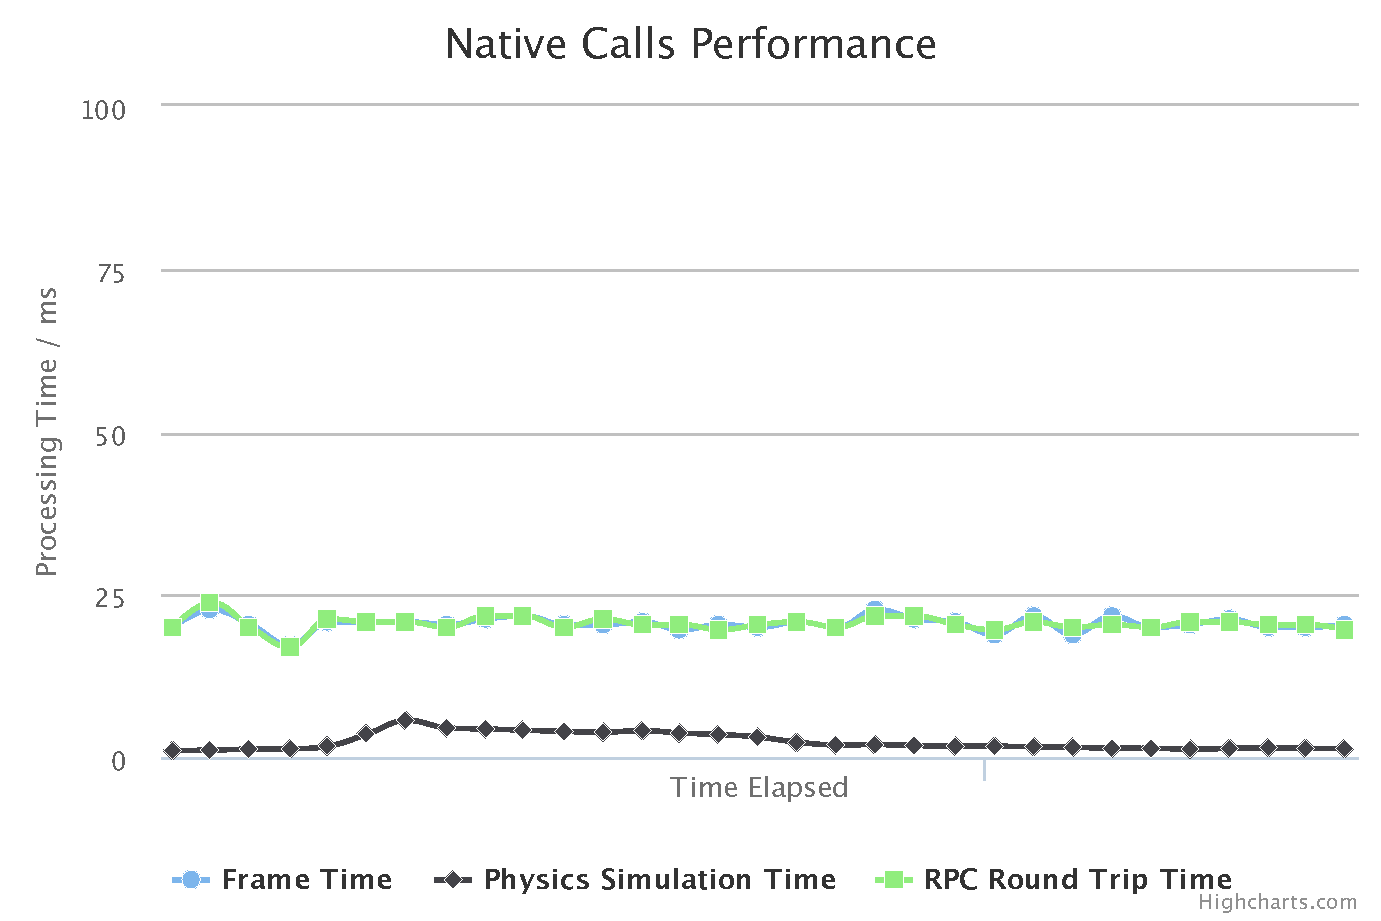
\includegraphics[width=\textwidth]{bulletdata_cylinder500_nc.pdf}
                % \caption{Using Native Calls}
                \label{fig:bulletdata_cylinder500_nc}
        \end{subfigure}%
        \\
        \begin{subfigure}[b]{\textwidth}
                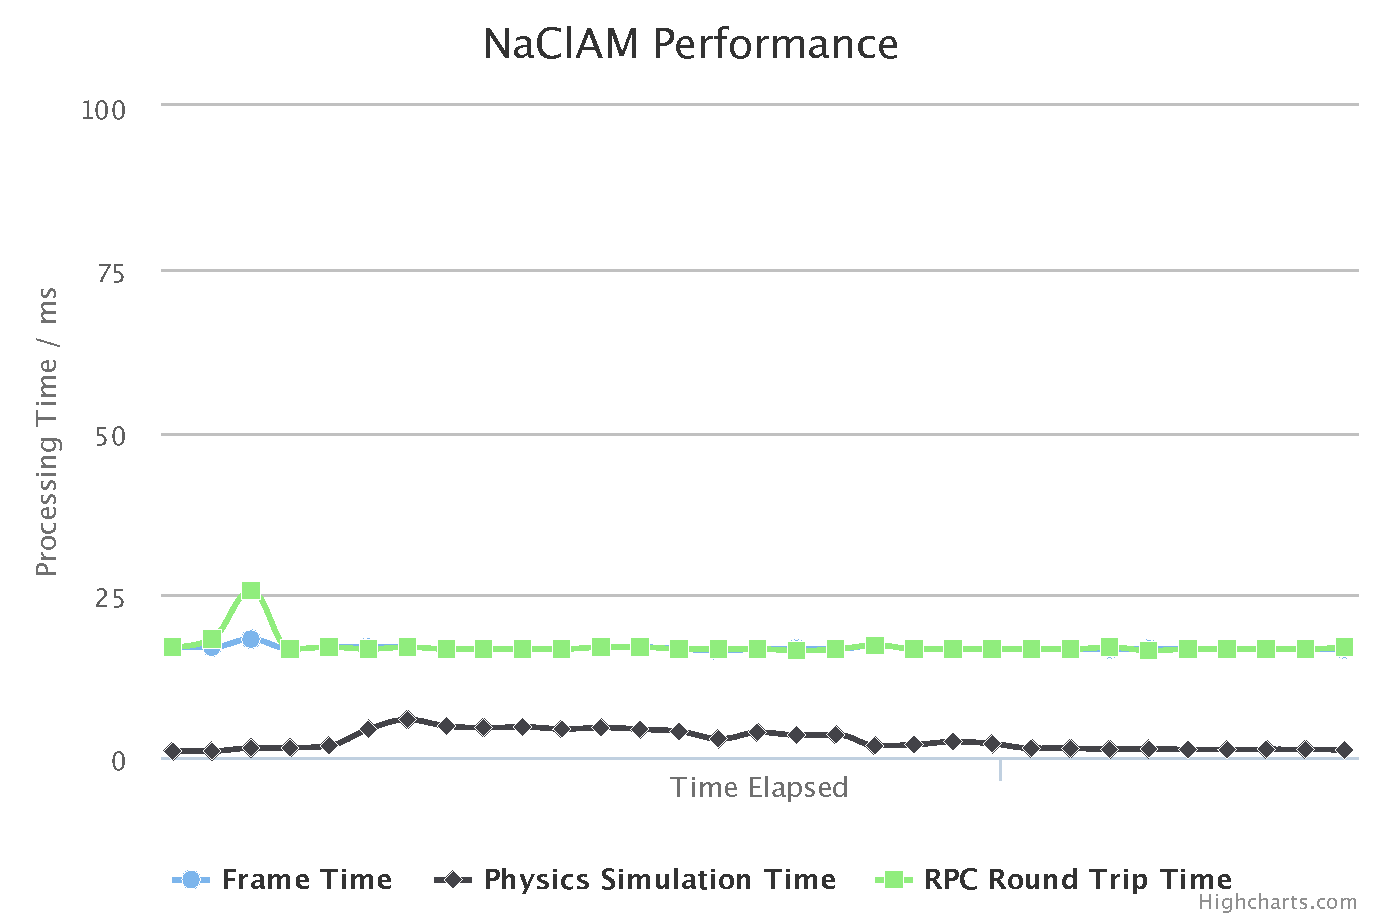
\includegraphics[width=\textwidth]{bulletdata_cylinder500_naclam.pdf}
                % \caption{Using NaClAM}
                \label{fig:bulletdata_cylinder500_naclam}
        \end{subfigure}
        \caption{The mean processing times per second over a period of 20 seconds, for Scene E: 500 cylinders. The two graphs show the results using the same scene but different implementations.}
        \label{fig:bullet_graph_cyl500}
\end{figure}

\begin{figure}
        \centering
        \begin{subfigure}[b]{\textwidth}
                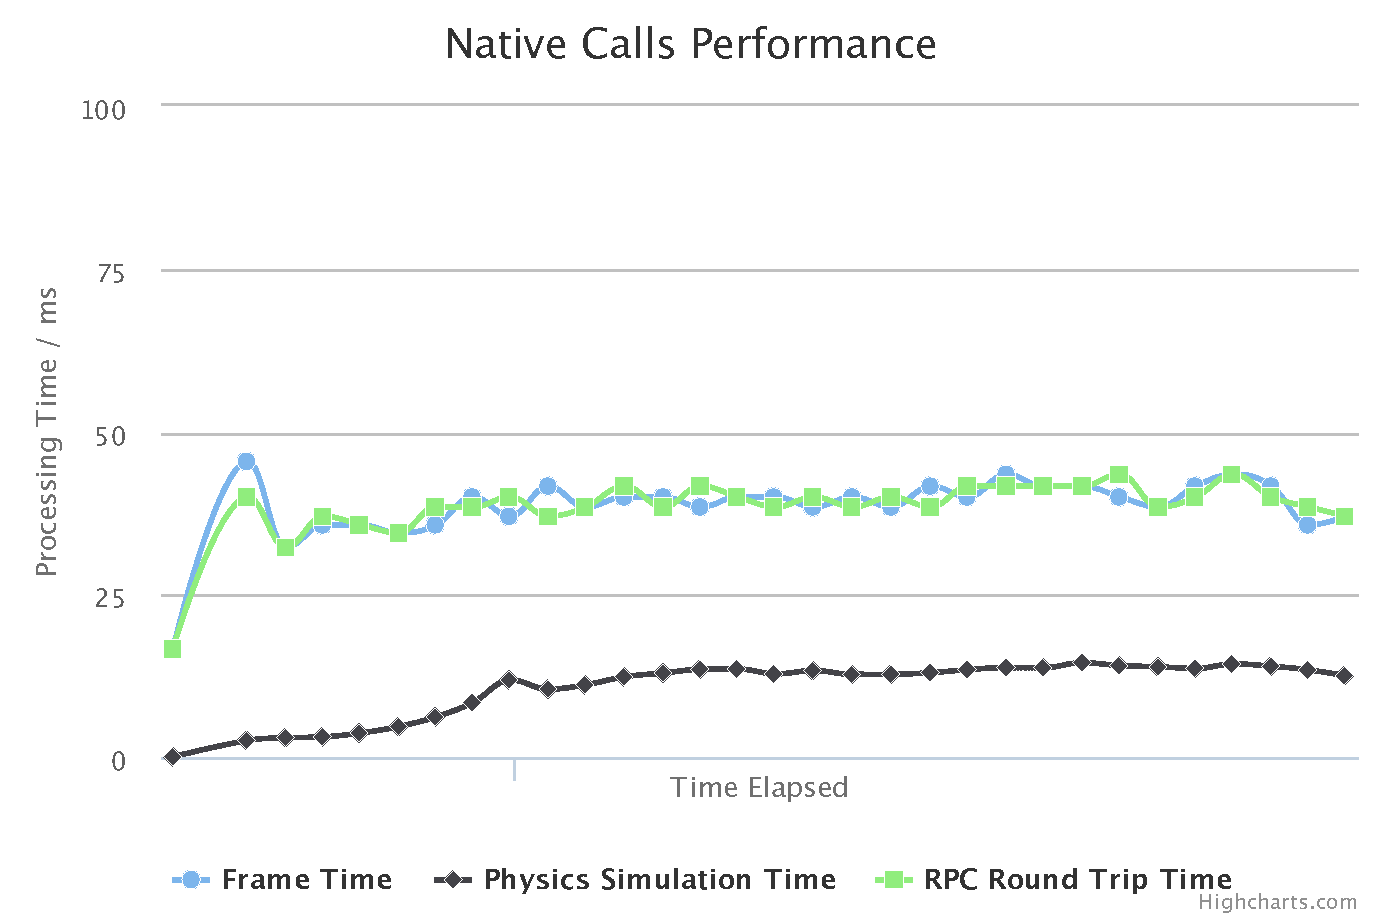
\includegraphics[width=\textwidth]{bulletdata_cube1000_nc.pdf}
                % \caption{Random Shapes}
                % \label{fig:random_shapes}
        \end{subfigure}
        \\
        \begin{subfigure}[b]{\textwidth}
                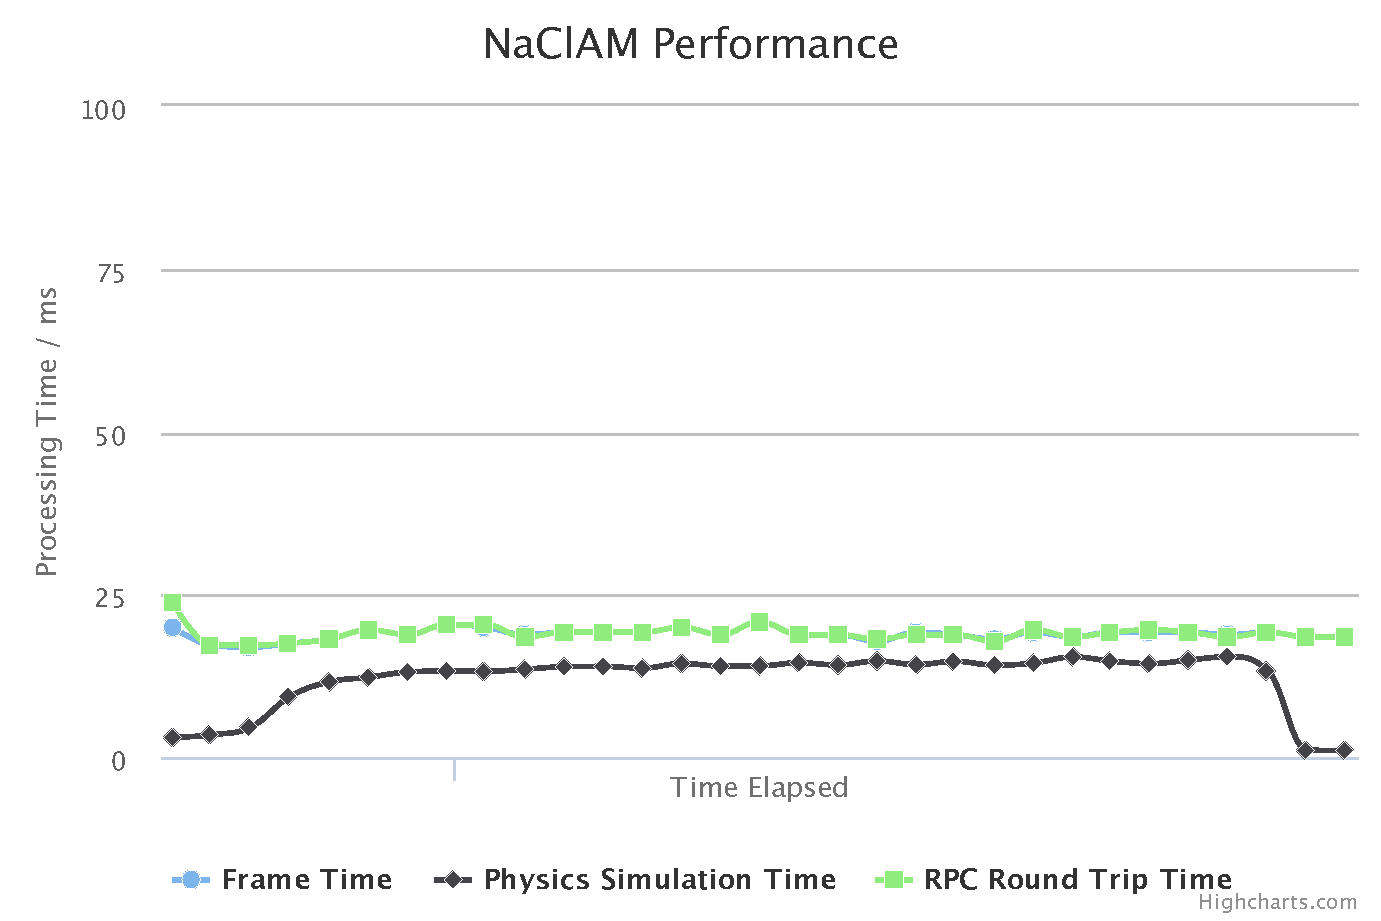
\includegraphics[width=\textwidth]{bulletdata_cube1000_naclam.pdf}
                % \caption{250 Cubes}
                % \label{fig:cubes_250}
        \end{subfigure}
        \caption{The mean processing times per second over a period of 20 seconds, for Scene F: 1000 cubes.}
        \label{fig:bullet_graph_cube1000}
\end{figure}

\begin{figure}
        \centering
        \begin{subfigure}[b]{\textwidth}
                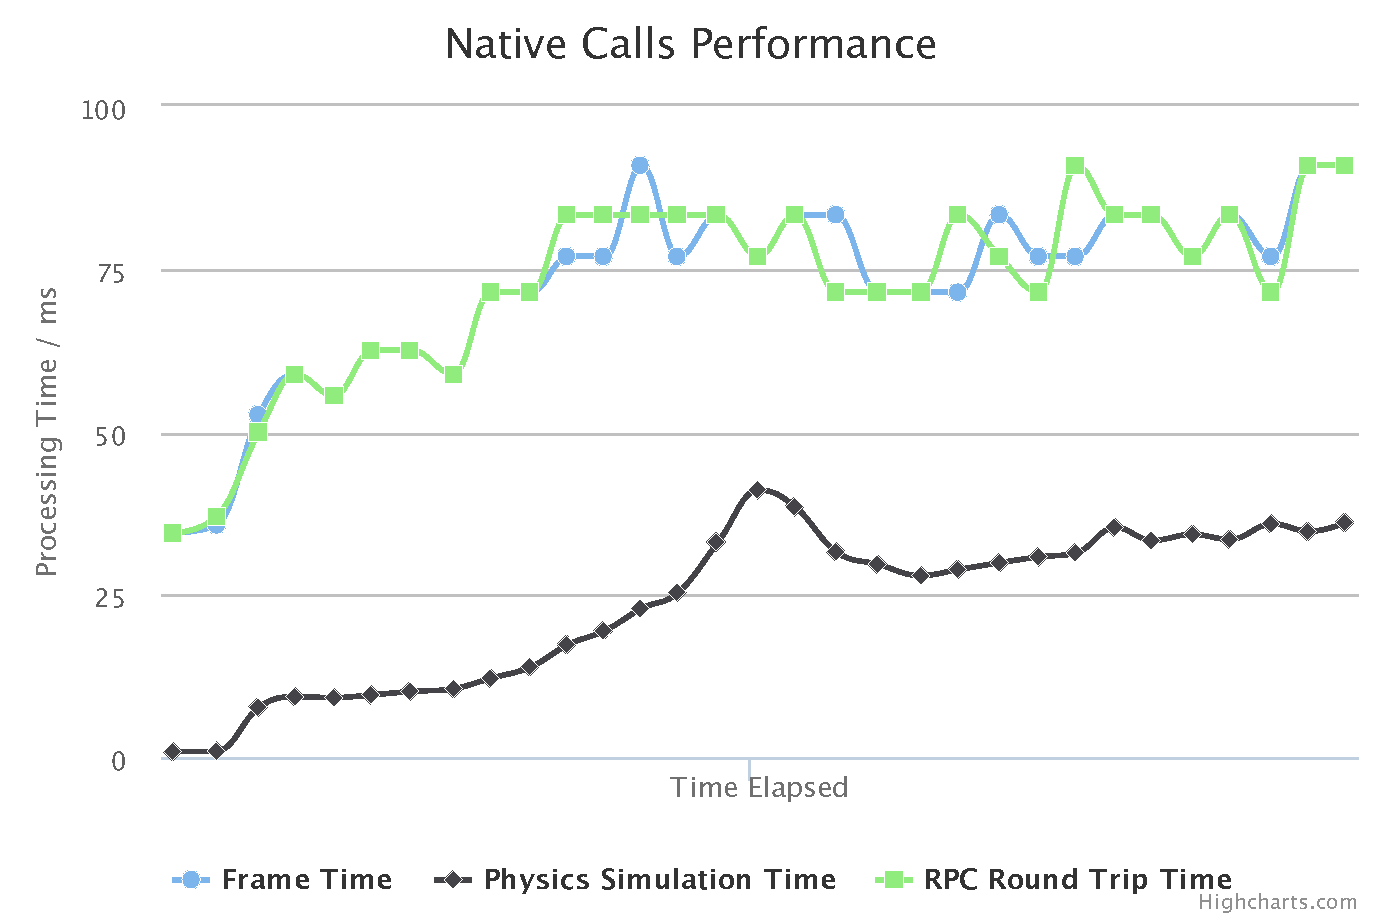
\includegraphics[width=\textwidth]{bulletdata_cube2000_nc.pdf}
                % \caption{500 Cylinders}
                % \label{fig:cylinders_500}
        \end{subfigure}%
        \\
        \begin{subfigure}[b]{\textwidth}
                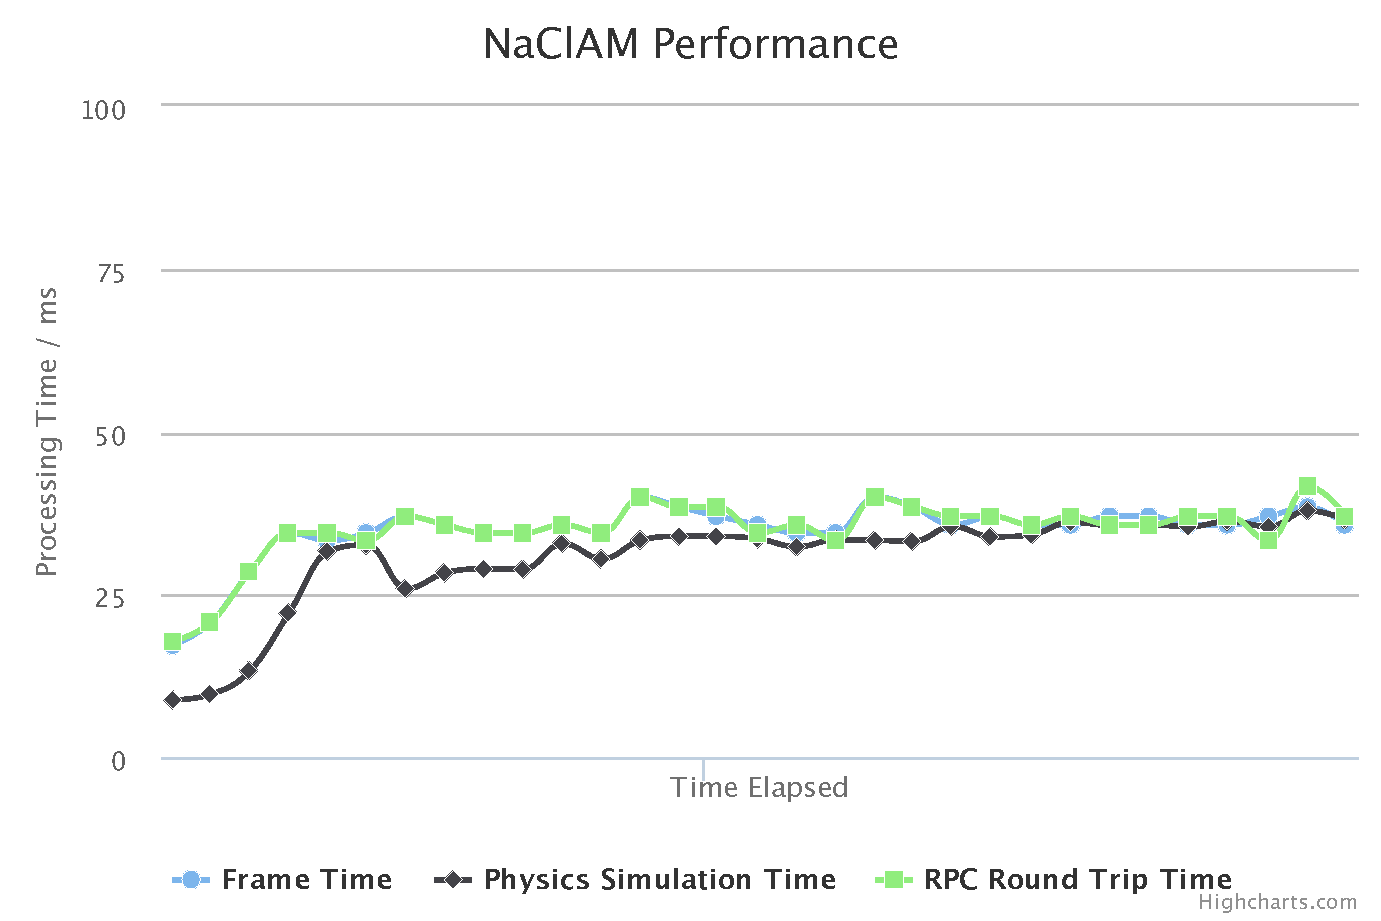
\includegraphics[width=\textwidth]{bulletdata_cube2000_naclam.pdf}
                % \caption{1000 Cubes}
                % \label{fig:cubes_1000}
        \end{subfigure}
        \caption{The mean processing times per second over a period of 20 seconds, for Scene G: 2000 cubes.}
        \label{fig:bullet_graph_cube2000}
\end{figure}

% subsubsection results_bullet_physics_performance (end)

\subsubsection{Analysis} % (fold)
\label{ssub:bullet_physics_performanceanalysis}
From the graphs and tables, we can obviously see how the performance impact of our framework gets higher and higher with more and more objects being sent. We can see how for large scenes such as 2000 cubes, the Native Calls implementation performs almost two times worse than the NaClAM implementation. However for smaller scenes, the two implementations have very similar performance.

From the graphs we can see how the Native Calls framework contributes to the performance impact. For example, in Figure \ref{fig:bullet_graph_cube2000}, the large space between the physics simulation time line and the RPC round trip time line is an indication that the framework is doing most of the processing in the RPC call, not the simulation. When we compare this to the NaClAM version in the same figure, it is clear that most of the processing happens in the physics simulation.

The most likely reason for these two observations is that the data marshalling on the C++ Native Calls RPC framework implementation negatively impacts the performance. In our implementation, the data is processed in O(n) time in order to convert the received \lstinline{pp::VarArray} array of objects into a \lstinline{std::vector} of \lstinline{struct}s. In section \ref{sec:performance_evaluation} (page \pageref{sec:performance_evaluation}), we find that converting WebIDL dictionaries is also quite slow, compared to converting an array of numbers. When we compare this to the NaClAM implementation, we can see that the NaClAM version has almost O(1) time, since the data is only being read and is shared between the module and JavaScript. This is explained in section \ref{sec:naclam} on page \pageref{sec:naclam}.

% subsubsection bullet_physics_performanceanalysis (end)


% subsection bullet_physics_performance (end)

\subsection{Oniguruma Regular Expressions Performance} % (fold)
\label{sub:oniguruma_regular_expressions_performance}
To get an insight of the performance of the oniguruma library for Native Client using Native Calls, we shall count the number of regular expression matches. We compare this to running the engine in Node JS server natively, and then using WebSockets to get functionality in the browser.

\subsubsection{Setup} % (fold)
\label{ssub:onig_performance_setup}
Again, the actual implementation of the library is discussed later on in the evaluation, in section \ref{sub:implementation_oniguruma_evaluation} on page \pageref{sub:implementation_oniguruma_evaluation}. In this section, we discuss how we measure the time it took to find all matches.

For the benchmark, we searched a large code base. We took part of the jQuery implementation in JavaScript and stored it in a string. We then performed regular expression searches on that string. The search string was 3467 characters. We split it into lines. For each line, we found all instances of \lstinline{"this"}, \lstinline{"var"}, \lstinline{"selector"}, and \lstinline{"window"} using regular expressions. In total, there was 237 matches, and each implementation gave the correct output. However, we measured the amount of time it took to find all these matches.

For the browser implementations (Native Calls and web sockets), we measure it using BenchmarkJS, to get an accurate running time, and a relative error margin. Using BenchmarkJS, we measured the time it took from initiating a request to receiving a response. BenchmarkJS performed the tests hundreds of times to get an accurate running time.

For the server implementation (using node.js natively on the server), we simply timed and performed all the searches 1000 times and got the mean of the running time.
% subsubsection onig_performance_setup (end)

\subsubsection{Results and comparison} % (fold)
\label{ssub:onig_results_and_comparison}
Table \ref{table:onig_time_taken} shows the results of running the benchmark application using Native Calls RPC and node-oniguruma.

\begin{table}[h]
\centering
\begin{tabular}{l|l}
\textbf{Method}                 & \textbf{Time Taken / s} \\ \hline
Native Calls                    &  0.709 $\pm$0.47\%  \\
node-oniguruma with web sockets &  0.375 $\pm$0.32\%  \\
node-oniguruma (native)         &  0.045                  
\end{tabular}
\caption{A comparison of the time taken to find all matches of a regular expression using different implementations}
\label{table:onig_time_taken}
\end{table}

% subsubsection onig_results_and_comparison (end)

\subsubsection{Analysis} % (fold)
\label{ssub:onig_analysis}
We can see that the node-oniguruma version performs much better. This is due to a number of reasons:
\begin{itemize}
  \item The node-oniguruma implementation is \emph{native}, in the sense that it uses JavaScript types directly. No marshalling nor transfer happens.
  \item The node.js V8 engine usually performs better than V8 in Chrome, as it is optimised for server side performance.
  \item The web socket implementation has a very simple runtime on both client and server sides. No error checking, type checking, etc. happens.
  \item Strings are the slowest primitive types to marshal, send and de-marshal in Native Calls. See section \ref{sec:performance_evaluation} for details.
\end{itemize}
% subsubsection onig_analysis (end)


% subsection oniguruma_regular_expressions_performance (end)
% section application_performance_evaluation (end)

\section{Framework Performance Evaluation} % (fold)
\label{sec:performance_evaluation}
We used the IDL file shown in Listing \ref{code_webidl_benchmarks} to test transfer and processing performance of individual operations:

\lstset{language=WebIDL,caption={WebIDL file used for benchmarking},label=code_webidl_benchmarks}
\begin{code}
dictionary dict {
  DOMString str;
  double d;
  boolean b;
};

dictionary nestedDict {
  DOMString topStr;
  double topD;
  boolean topB;
  dict nested;
};

interface Benchmark{
  long bench_long(long v);
  double bench_double(double v);
  DOMString bench_DOMString(DOMString v);
  dict bench_dict(dict v);
  nestedDict bench_nestedDict(nestedDict v);

  sequence<long> bench_seq_long(sequence<long> v);
  sequence<double> bench_seq_double(sequence<double> v);
  sequence<DOMString> bench_seq_DOMString(sequence<DOMString> v);
  sequence<dict> bench_seq_dict(sequence<dict> v);
  sequence<nestedDict> bench_seq_nestedDict(sequence<nestedDict> v);
};
\end{code}

We will use the generated RPC library to test the framework's performance. We will do this by making RPC calls and measuring how long it takes.

\subsection{Round trip performance}\label{round-trip-performance}

We measure the number of round trips performed in one second (round trips per second, RT/s).

One round trip corresponds to a full remote procedure call, starting from JavaScript, reaching the target function, returning from the function, and going back to the JavaScript. This is illustrated in Figure \ref{fig:rpc_roundtrip}.


\begin{figure}
    \centering
    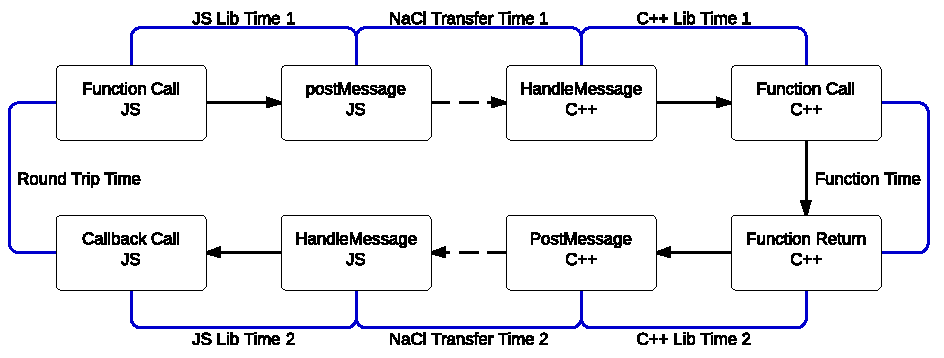
\includegraphics[width=1\textwidth]{RoundTrip.pdf} 
    \caption{A depiction of the round trip time from JavaScript to C++}
    \label{fig:rpc_roundtrip}
\end{figure}


\begin{table}[h]
\centering
\begin{tabular}{l|lll}
\textbf{Type}       & \textbf{Mean RT/s} & \textbf{Uncertainty} & \textbf{Number of runs} \\ \hline
\textbf{long}       & 418                & $\pm$1.79\%              & 56                      \\
\textbf{double}     & 423                & $\pm$2.08\%              & 48                      \\
\textbf{DOMString}  & 420                & $\pm$1.25\%              & 43                      \\
\textbf{dict}       & 415                & $\pm$2.39\%              & 44                      \\
\textbf{nestedDict} & 385                & $\pm$1.29\%              & 47                     
\end{tabular}
\caption{Round trip performance of sending a single parameter}
\label{table:roundtrip_single_param}
\end{table}


\begin{table}[h]
\centering
\begin{tabular}{l|lllll}
\multirow{2}{*}{\textbf{Array Length}} & \multicolumn{5}{l}{\textbf{Round trips per second}}                                        \\
                                       & \textbf{long} & \textbf{double} & \textbf{DOMString} & \textbf{dict} & \textbf{nestedDict} \\ \hline
\textbf{10}                            & 403               & 403                 & 378                    & 317               & 244                     \\
\textbf{45}                            & 379               & 384                 & 309                    & 182               & 112                     \\
\textbf{100}                           & 354               & 347                 & 234                    & 110               & 60.07                   \\
\textbf{450}                           & 237               & 235                 & 102                    & 32.82             & 15.83                   \\
\textbf{1000}                          & 163               & 160                 & 55.41                  & 15.39             & 7.43                    \\
\textbf{4500}                          & 49.39             & 48.93               & 14.60                  & 3.62              & 1.68                    \\
\textbf{10000}                         & 24.68             & 24.50               & 6.62                   & 1.62              & 0.75                    \\
\textbf{45000}                         & 5.99              & 5.98                & 1.28                   & 0.33              & 0.15                   
\end{tabular}
\caption{Round trip performance for arrays of different lengths and types}
\label{table:roundtrip_array}
\end{table}

Tables \ref{table:roundtrip_array} and \ref{table:roundtrip_single_param} show the number of round trips performed in a second for RPC calls with a single parameter and different array lengths. To compare these times, Figure \ref{fig:arraylength-time-plot} shows a column chart visualisation of the data.

\begin{figure}
    \centering
    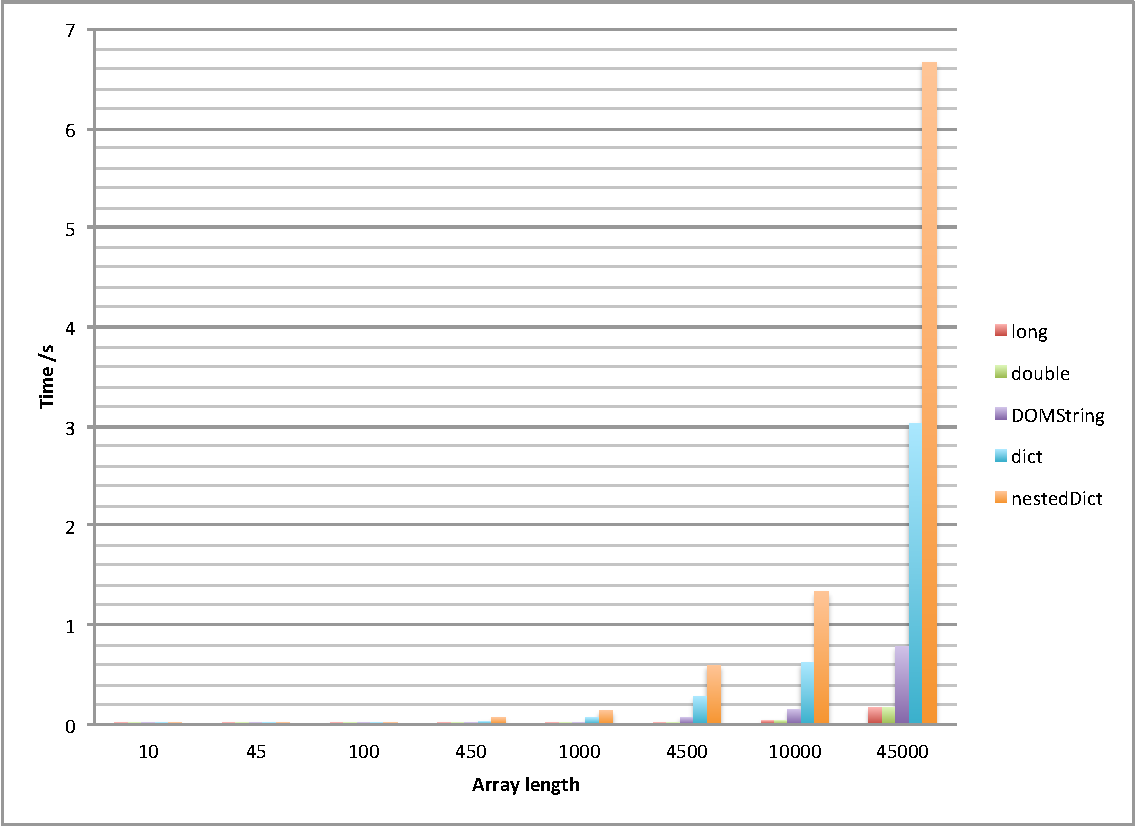
\includegraphics[width=1\textwidth]{arraylength-time-plot.pdf} 
    \caption{The round trip time for arrays of different lengths and types}
    \label{fig:arraylength-time-plot}
\end{figure}


\begin{figure}
    \centering
    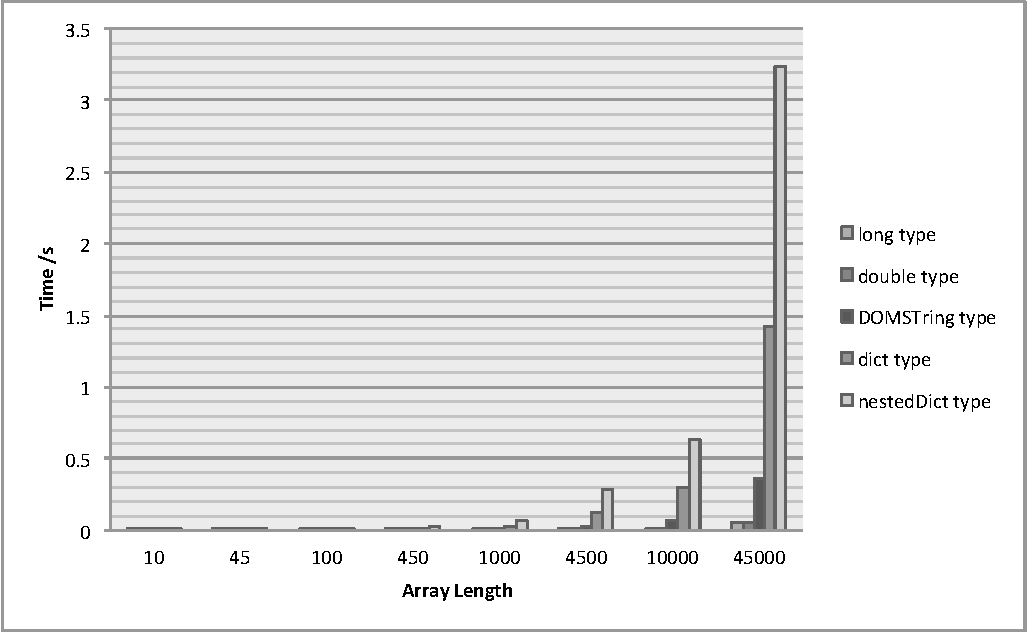
\includegraphics[width=1\textwidth]{arraylength-time-cpp-plot.pdf} 
    \caption{The C++ library time for arrays of different lengths and types}
    \label{fig:arraylength-time-cpp-plot}
\end{figure}



\subsection{C++ Library Time}\label{c-library-time}

We measure the number of microseconds taken to handle a RPC call. This is the time it takes to detect it is an RPC call, extract parameters, convert them, find the method, call it, pack the result, and post the message back to JS.

The results are measured and averaged for the same runs that were performed above. Tables \ref{table:cpp_lib_time_single_param} and \ref{table:cpp_lib_time_arrays} show the results, and Figure \ref{fig:arraylength-time-cpp-plot} shows a visualisation of the data.


\begin{table}[h]
\centering
\begin{tabular}{l|ll}
\textbf{Type}       & \textbf{Mean lib time/$\mu$s} & \textbf{Uncertainty (1 sd)} \\ \hline
\textbf{long}       & 106                       & 18                          \\
\textbf{double}     & 104                       & 17                          \\
\textbf{DOMString}  & 104                       & 18                          \\
\textbf{dict}       & 136                       & 23                          \\
\textbf{nestedDict} & 180                       & 28                         
\end{tabular}
\caption{Mean C++ library time for sending and receiving single parameters of different types}
\label{table:cpp_lib_time_single_param}
\end{table}


\begin{table}[h]
\centering
\begin{tabular}{l|lllll}
\multirow{2}{*}{\textbf{Array Length}} & \multicolumn{5}{l}{\textbf{Time / $\mu$s}}                                                                             \\
                                       & \textbf{long} & \textbf{double} & \textbf{DOMSTring} & \textbf{dict} & \textbf{nestedDict} \\ \hline
\textbf{10}                            & 125                & 126                  & 197                     & 453                & 861                      \\
\textbf{45}                            & 169                & 163                  & 484                     & 1513               & 3273                     \\
\textbf{100}                           & 243                & 246                  & 906                     & 3445               & 7010                     \\
\textbf{450}                           & 705                & 704                  & 3735                    & 13629              & 28198                    \\
\textbf{1000}                          & 1276               & 1355                 & 7607                    & 29582              & 63494                    \\
\textbf{4500}                          & 5548               & 5564                 & 30485                   & 132122             & 292828                   \\
\textbf{10000}                         & 11283              & 11376                & 68444                   & 301438             & 632956                   \\
\textbf{45000}                         & 50532              & 50843                & 359134                  & 1418792            & 3242286                  \\
\textbf{100000}                        & 104087             & 114020               & 799743                  & 3319250            & 7347985                 
\end{tabular}
\caption{Mean C++ library time for sending and receiving arrays of different lengths and types}
\label{table:cpp_lib_time_arrays}
\end{table}

\subsection{JS Library performance}\label{js-library-performance}

The JS library performance \textbf{without} client-side type validation has also been measured, however its performance impact is negligible. The slowest benchmark was found to take approx 3 microseconds (269,253 ops/sec $\pm$  1.90\%).

\subsection{Analysis}\label{analysis}

From the data, we can see that for small types, the most contributing factor to performance is the browser (e.g.~event system, etc.) and PPAPI libraries (how PPAPI implements postMessage). For example, sending a single long type takes 2392.34 microseconds (.002 seconds), but our library only spends 105.5 microseconds processing the call (less than 5\% of the time).

For large and complicated data, the impact of using the library becomes higher and higher. For example, sending 45000 nested objects (which are actually quite simple) has a total round-trip time of 6.67s, and a whole 3.24 seconds of this is spent in our library (i.e.~half the time).

The most likely reason for this is that the C++ library takes O(n) time to process the data in order to marshal it, by converting it from a \lstinline{pp::VarArray} into a \lstinline{std::vector}.

We also notice that the DOMString and Dictionary types are the slowest to marshal and de-marshal. One reason for this could be that number types have a standard representation so perhaps the PPAPI was able to improve how they are transferred, whilst the string types and dictionary types would need marshalling even by the PPAPI. One obvious reason for why the dictionary types take longer to marshal is that they contain multiple types, each type is individually marshalled. So sending a dictionary with multiple keys and values is almost equivalent to sending multiple values separately.

% section performance_evaluation (end)
\newpage

\section{Usability Evaluation} % (fold)
\label{sec:usability_evaluation}
To get some insight as to how usable and useful the library and generator is, we analyse the number of lines the developer would need to write to build the same application. We take a look at two different applications: a bullet physics simulation which uses the C++ module to calculate simulation steps, and a regular expression library which uses a native module to do execute regular expressions. The table below shows how many lines the developer had to write to achieve the same program.

\subsection{Implementation: Bullet} % (fold)
\label{sub:implementation_bullet_evaluation}
We use the IDL shown in Listing \ref{code_bullet_idl} as our interface. This allows us to send normal JavaScript objects to the C++ implementation, and in C++, the dictionaries are automatically marshalled as structs.

The rest of the implementation is taken from the original implementation. This is basically a static object which holds all the information about the scene, allows loading a scene, and calculates simulation steps, all using the Bullet Physics library.
% subsection implementation_bullet_evaluation (end)

\subsection{Implementation: Oniguruma} % (fold)
\label{sub:implementation_oniguruma_evaluation}
We use the IDL shown in Listing \ref{code_ong_idl}. Again, the rest of the implementation is taken from the node-oniguruma original project. There is a critical difference though, which is to do with the object-oriented nature of the regular expressions. To implement this, we have a static map of Scanner ids to C++ references to Scanner objects. RPC requests call the C++ class methods, using the id to to get the actual instance. An example of how this works is shown in the C++ Listing \ref{code_rpc_oop_cpp}. 
% subsection implementation_oniguruma_evaluation (end)

\lstset{language=C,caption={WebIDL for Bullet},label=code_bullet_idl}
\begin{code}
dictionary XYZ{
	float x;
	float y;
	float z;
};

dictionary Cube{
	DOMString name;
	float wx;
	float wy;
	float wz;
};

dictionary Convex{
	DOMString name;
	sequence<XYZ> points;
};

// Sphere, Cylinder, and Body  defined similarly.

dictionary Scene{
	sequence<Cube> cubes;
	sequence<Convex> convices;
	sequence<Sphere> spheres;
	sequence<Cylinder> cylinders;
	sequence<Body> bodies;
};

dictionary SceneUpdate{
	sequence<float> transform;
	unsigned long long delta;	
};

interface BulletInterface {
	double LoadScene(Scene scene);
	SceneUpdate StepScene(XYZ rayTo, XYZ rayFrom);
	boolean PickObject(double index, XYZ pos, XYZ cpos);
	boolean DropObject();
};
\end{code}


\lstset{language=C,caption={WebIDL for the Oniguruma implementation},label=code_ong_idl}
\begin{code}
dictionary CaptureIndex{
	unsigned long start;
	unsigned long end;
	unsigned long length;
	unsigned long index;
};

dictionary OnigMatch{
	unsigned long index;
	sequence<CaptureIndex> captureIndices;
};

interface Scanner{
	unsigned long newScanner(sequence<DOMString> patterns);
	OnigMatch findNextMatch(unsigned long scannerID, DOMString string,
	                                     unsigned long startPosition);
};
\end{code}

\lstset{language=C++,caption={Wrapping C++ instance methods with RPC functions, in the Oniguruma implementation},label=code_rpc_oop_cpp}
\begin{code}
uint32_t newScanner( std::vector<std::string> patterns){
        return OnigScanner::newInstance(patterns);
}

OnigMatch findNextMatch( uint32_t scannerID,  std::string string,  
                                              uint32_t startPosition){
        OnigScanner* scanner = OnigScanner::getInstance(scannerID);
        return scanner->findNextMatch(string, startPosition);
}
\end{code}
\newpage
\subsection{Results: Bullet} % (fold)
\label{sub:evaluation_usability_bullet}
\begin{table}[h]
\begin{tabular}{llll}
\#lines                    & Original & Native Calls & Difference \\ \cline{2-4} 
\multicolumn{1}{l|}{C++}   & 404      & 331          &  73        \\
\multicolumn{1}{l|}{JS}    & 979      & 811          &  168       \\
\multicolumn{1}{l|}{IDL}   & 0        & 54           &  -54       \\
\multicolumn{1}{l|}{Total} & 1383     & 1196         &  187
\end{tabular}
\end{table}

We can see a total of 187 lines were saved by using the Native Calls library and generators. In the C++ code, most of these differences occurred because the NaClAM version required the user to marshal and de-marshal the messages manually. For example, Listings \ref{code_pickobject_nc} and \ref{code_pickobject_naclam} shows how both implementations handle the \lstinline{PickObject} RPC call.

\lstset{language=C++,caption={Native Calls Implementation of PickObject},label=code_pickobject_nc}
\begin{code}
bool PickObject(double index, XYZ pos, XYZ cpos) {
  if (!bulletScene.dynamicsWorld) {
    return false;
  }
  index++;
  if (index < 0 || 
       index >= bulletScene.dynamicsWorld->getNumCollisionObjects()) {
    bulletScene.pickedObjectIndex = -1;
    return false;
  }
  bulletScene.pickedObjectIndex = index;
  bulletScene.addPickingConstraint(btVector3(cpos.x, cpos.y, cpos.z), 
                                      btVector3(pos.x, pos.y, pos.z));
  return true;
}
\end{code}


\lstset{language=C++,caption={NaClAM implementation of PickObject},label=code_pickobject_naclam}
\begin{code}
void handlePickObject(const NaClAMMessage& message) {
  if (!scene.dynamicsWorld) {
    return;
  }
  const Json::Value& root = message.headerRoot;
  const Json::Value& args = root["args"];
  const Json::Value& objectTableIndex = args["index"];
  const Json::Value& pos = args["pos"];
  const Json::Value& cpos = args["cpos"];
  float x = pos[0].asFloat();
  float y = pos[1].asFloat();
  float z = pos[2].asFloat();
  float cx = cpos[0].asFloat();
  float cy = cpos[1].asFloat();
  float cz = cpos[2].asFloat();
  int index = objectTableIndex.asInt();
  index++;
  if (index < 0 || 
             index >= scene.dynamicsWorld->getNumCollisionObjects()) {
    scene.pickedObjectIndex = -1;
    return;
  }
  scene.pickedObjectIndex = index;
  scene.addPickingConstraint(btVector3(cx, cy, cz), btVector3(x,y,z));
  NaClAMPrintf("Picked \%d\n", scene.pickedObjectIndex);
}
\end{code}

In the JavaScript code, most of the lines saved were type checking code and separate functions for the RPC calls and handlers. For example, the whole of \lstinline{world.js} (140 lines) is type checking code similar to Listing \ref{code_js_typechecking_naclam}. Notice how this doesn't even check the actual types, it just checks if the fields are defined. On the other hand, the generated Native Calls library produces full, structure recursive, convenient type checking without extra effort from the developer. Listing \ref{code_naclam_loadworld} shows an example of how separate handlers had to be written for the NaClAM implementation, while Listing \ref{code_nc_loadworld} shows how the same effect is achieved by the use of callbacks.

\lstset{language=C,caption={NaClAM implementation's JavaScript type checking example},label=code_js_typechecking_naclam}
\begin{code}
function verifyCubeDescription(shape) {
  if (shape['wx'] == undefined) {
    return false;
  }
  if (shape['wy'] == undefined) {
    return false;
  }
  if (shape['wz'] == undefined) {
    return false;
  }
  return true;
}
\end{code}

\lstset{language=C,caption={NaClAM implementation of requests and response handlers},label=code_naclam_loadworld}
\begin{code}
// somewhere in scene.js... 
function loadWorld(worldDescription) {
  clearWorld();
  //... some JS implementation
  NaClAMBulletLoadScene(worldDescription); // RPC request
  lastSceneDescription = worldDescription;
}

// somewhere in NaClAMBullet.js...
function NaClAMBulletInit() {
  aM.addEventListener('sceneloaded', NaClAMBulletSceneLoadedHandler);
  // other handlers
}

function NaClAMBulletLoadScene(sceneDescription) {
  aM.sendMessage('loadscene', sceneDescription);
}

function NaClAMBulletSceneLoadedHandler(msg) {
  console.log('Scene loaded.');
  console.log('Scene object count = ' + msg.header.sceneobjectcount);
}
\end{code}

\lstset{language=C,caption={Native Calls Implementation of requests and response handlers},label=code_nc_loadworld}
\begin{code}
function loadWorld(worldDescription, callback ) {
  clearWorld();
  //... some JS implementation
  bullet.BulletInterface.LoadScene(rpcScene, function(result){
    console.log("Scene loaded "+ result);
    if(callback)callback();
  });
  lastSceneDescription = worldDescription;
}
\end{code}

We can see that for both the JavaScript and C++ developer, using Native Calls saves a lot of time. The examples also show how the developer does not need to get used to another paradigm (i.e. using listeners, requests, and handlers) or library (i.e. JsonCpp). Instead, using Native Calls, the developer on both JavaScript and C++ can focus on the main logic of the actual native module!

% subsection evaluation_usability_bullet (end)

\subsection{Results: Oniguruma} % (fold)
\label{sub:evaluation_usability_oniguruma}
\begin{table}[h]
\begin{tabular}{llll}
\#lines                    & Original & Native Calls & Difference \\ \cline{2-4} 
\multicolumn{1}{l|}{C++}   & 666      & 601          &  65        \\
\multicolumn{1}{l|}{JS}    & 100      & 134          &  -34       \\
\multicolumn{1}{l|}{IDL}   & 0        & 15           &  -15       \\
\multicolumn{1}{l|}{Total} & 766      & 750          &  16
\end{tabular}
\end{table}

Note: the original implementation used \emph{CoffeeScript}, we used the CoffeeScript compiler to get the equivalent JavaScript code. The generated JavaScript code is what is counted - and although it is computer generated, it maps directly to human-readable JavaScript that would have been written. We consider this fair when we compare the number of lines, as CoffeeScript introduces a lot of \emph{syntax sugar} which can greatly reduce the number of lines in JavaScript. The number of CoffeeScript lines in the original implementation is 51.

We can see that only a few number of lines are saved in the Oniguruma implementation. This is because of the fact that Native Calls does not currently support object oriented RPC. The JavaScript developer lost quite a few lines because of this. We needed to create a class that makes the RPC calls and keeps references to objects in the C++ code. Listing \ref{code_onig_js_rpc_class} shows this. The \lstinline{_whenScannerReady} member function allows calling different RPC functions with a scannerID. Scanners are instantiated dynamically in the C++ using the \lstinline{newScanner} RPC call. All member functions then take in an extra parameter, the ID, which is used to find the instance in the C++ code.

We compare this to the node-oniguruma implementation. Here, the C++ implementation extends JavaScript, so a C++ object corresponds directly to a JavaScript object. This is explained in the related work section \ref{sec:node_js_c_bindings} on page \pageref{sec:node_js_c_bindings}.

\lstset{language=C,caption={Augmenting RPC: Wrapping RPC methods with a JS class},label=code_onig_js_rpc_class}
\begin{lstlisting}
function OnigScanner(sources){
  this.ready = false;
  this.scannerID = -1;
  this.sources = sources;
  this.scanner = scanner; // the RPC interface
}

OnigScanner.prototype._whenScannerReady = function(callback){
  var thisRef = this;
  if(this.ready){
    // call straightaway.
    if(typeof callback == "function"){
      callback.apply(this);
    }
  } else {
    // new scanner then call. does RPC request
    this.scanner.newScanner(this.sources, function(scannerID){
      thisRef.ready = true;
      thisRef.scannerID = scannerID;
      if(typeof callback == "function"){
        callback.apply(thisRef);
      }
    });
  }
};

OnigScanner.prototype.findNextMatch = function(string, startPosition, 
                                                           callback) {
  this._whenScannerReady(function(){
    var thisRef = this;
    // RPC with scannerID which is used to find the C++ instance
    this.scanner.findNextMatch(this.scannerID, string, startPosition, 
                                                      function(match){
      if(match.captureIndices.length == 0){
        match = null;
      }
      if(match != null){
        match.scanner = thisRef;
      }
      if(typeof callback == "function"){
        callback(match);
      }
    });
  });
};
\end{lstlisting}

% subsection evaluation_usability_oniguruma (end)

% section usability_evaluation (end)
\newpage

\section{Evaluation Conclusion} % (fold)
\label{sec:eval_usability_conclusion}
After looking at two different applications, we can see that for static or singleton-based applications, such as the bullet physics application, the Native Calls library and generators saves a lot of development time and provides a natural, straight forward method of implementing a C++ library usable from JavaScript. However, for object oriented applications, we find that the JavaScript and C++ developer must think about implementing low level details such as instance look up in order to give a object oriented RPC system.

As for performance, we find that the performance impact is negligible for RPC calls with little data. The impact increases with increasing data size.

This makes using Native Calls perfect for singleton-based applications which send and receive little data, while a trade-off must be made for object-oriented applications or applications that send and receive large data.
% section eval_usability_conclusion (end)
 
\chapter{Conclusion}
\label{Chapter6}
\lhead{Chapter 6. \emph{Conclusion}} 
%solutions, challenges, outcomes

In this project, we have provided a solution for writing high performance JavaScript applications that use a C++ Native Client modules, in a way that is natural to both the JavaScript developer and C++ developer. To do this, we provide a code generator that produces C++ and JavaScript code in a package that the C++ developer can change and tweak for performance and feature extension. The C++ developer will have to write an interface in WebIDL, then the generator will produce all the boiler-plate code for both JavaScript and C++.

The main challenges were how to map WebIDL types and interfaces to C++ and JavaScript language features, and using a parser to produce human readable JavaScript and C++ code. Other challenges included using PostMessage as a transport layer for a layered RPC framework on both JavaScript and C++, as well as creating a testing framework and a build system based on the Native Client examples to efficiently build and test C++ Native Client modules in the browser.

In the end, we developed the generator and framework and wrote demo applications to test its usability and performance. We concluded that the framework performed well when little data is passed to the RPC functions, however, had a larger performance impact when large amounts of data are sent and received. We found that the code generator saved a lot of development time when compared to previous methods of implementing the same application, but developing object oriented RPC functionality required some more time.

\newpage
\section{Future Work} % (fold)
\label{sec:future_work}
\begin{itemize}
	\item Provide C++ to JavaScript RPC. Whilst we originally set out to provide a multi-directional RPC framework, because of time constraints this was not possible and only JavaScript to C++ RPC was implemented. However, implementing RPC in the other direction is symmetrical in most cases, as several layers including transport and RPC will remain the same.
	\item Improve performance by sending binary data when we can. In section \ref{sec:future_extensions} on page \pageref{sec:future_extensions}, we mentioned some design considerations and possible implementation of sending binary data when an array of contiguous number types are sent. This will greatly improve performance since binary data is shared between JavaScript and C++.
	\item Experiment with different RPC protocols and data types, such as Google Protocol Buffers to see if a performance improvement can be achieved. Because of our layered approach to RPC, this should be feasible and could provide some interesting results.
	\item Improve performance by allowing the RPC framework to spawn a new thread per request, thus allowing concurrent RPC calls.
	\item Object oriented generated code. For the evaluation, we showed how it is possible to create an object oriented RPC library by wrapping the RPC calls in JavaScript classes which hold a C++ instance identifier. One future extension to the project would be to allow these classes to be generated automatically.
	\item Produce a JavaScript fall-back when Native Client is not supported in the browser. This can be done using PepperJS\cite{pepperjs}, a library by Google that uses emscripten\cite{emscripten} to transpile machine code produced by the Native Client compilers, into JavaScript code.
\end{itemize}
% section future_work (end) 


%----------------------------------------------------------------------------------------
%	THESIS CONTENT - APPENDICES
%----------------------------------------------------------------------------------------

% \addtocontents{toc}{\vspace{2em}} % Add a gap in the Contents, for aesthetics

% \appendix % Cue to tell LaTeX that the following 'chapters' are Appendices

% % Include the appendices of the thesis as separate files from the Appendices folder
% % Uncomment the lines as you write the Appendices

% % Appendix A

\chapter{Native Calls Getting Started Guide}
\label{AppendixA} 

\lhead{Appendix A. \emph{Native Calls Getting Started Guide}}
The following pages show the getting started tutorial as seen on GitHub. 
TODO: Move this into end of design and implementation section, as a main report body.


% \includepdf[pages=-]{getting-started.pdf}
% %\input{Appendices/AppendixB}
% %\input{Appendices/AppendixC}

% \addtocontents{toc}{\vspace{2em}} % Add a gap in the Contents, for aesthetics

% \backmatter

%----------------------------------------------------------------------------------------
%	BIBLIOGRAPHY
%----------------------------------------------------------------------------------------

\label{Bibliography}

\lhead{\emph{Bibliography}} % Change the page header to say "Bibliography"

\bibliographystyle{unsrtnat} % Use the "unsrtnat" BibTeX style for formatting the Bibliography

\bibliography{Bibliography} % The references (bibliography) information are stored in the file named "Bibliography.bib"

\end{document}
